%\SweaveUTF8
\documentclass[aspectratio=43]{beamer}
\usepackage{Sweave}

\usetheme{default}
% Slide setup, colour independent

\usepackage{amsmath,amssymb,amsthm}
\usepackage[utf8]{inputenc}
\usepackage{colortbl}
\usepackage{bm}
\usepackage{xcolor}
\usepackage{dsfont}
\usepackage{setspace}
%\usepackage{subfigure}
% To use \ding{234} and the like
\usepackage{pifont}
% To cross reference between slide files
\usepackage{zref-xr,zref-user}
% Use something like
% \zexternaldocument{fileI}
% in the tex files. And cite using \zref instead of \ref

% Fields and the like
\def\IC{\mathbb{C}}
\def\IF{\mathbb{F}}
\def\II{\mathbb{I}}
\def\IJ{\mathbb{J}}
\def\IM{\mathbb{M}}
\def\IN{\mathbb{N}}
\def\IP{\mathbb{P}}
\def\IR{\mathbb{R}}
\def\IZ{\mathbb{Z}}
\def\11{\mathds{1}}


% Bold lowercase
\def\ba{\mathbf{a}}
\def\bb{\mathbf{b}}
\def\bc{\mathbf{c}}
\def\bd{\mathbf{d}}
\def\be{\mathbf{e}}
\def\bf{\mathbf{f}}
\def\bh{\mathbf{h}}
\def\bi{\mathbf{i}}
\def\bj{\mathbf{j}}
\def\bk{\mathbf{k}}
\def\bn{\mathbf{n}}
\def\bp{\mathbf{p}}
\def\br{\mathbf{r}}
\def\bs{\mathbf{s}}
\def\bu{\mathbf{u}}
\def\bv{\mathbf{v}}
\def\bw{\mathbf{w}}
\def\bx{\mathbf{x}}
\def\by{\mathbf{y}}
\def\bz{\mathbf{z}}

% Bold capitals
\def\bB{\mathbf{B}}
\def\bD{\mathbf{D}}
\def\bE{\mathbf{E}}
\def\bF{\mathbf{F}}
\def\bG{\mathbf{G}}
\def\bI{\mathbf{I}}
\def\bL{\mathbf{L}}
\def\bN{\mathbf{N}}
\def\bP{\mathbf{P}}
\def\bR{\mathbf{R}}
\def\bS{\mathbf{S}}
\def\bT{\mathbf{T}}
\def\bX{\mathbf{X}}

% Bold numbers
\def\b0{\mathbf{0}}

% Bold greek
\bmdefine{\bmu}{\bm{\mu}}
\def\bphi{\bm{\phi}}
\def\bvarphi{\bm{\varphi}}
\def\bPi{\bm{\Pi}}
\def\bGamma{\bm{\Gamma}}

% Bold red sentence
\def\boldred#1{{\color{red}\textbf{#1}}}
\def\defword#1{{\color{orange}\textbf{#1}}}

% Caligraphic letters
\def\A{\mathcal{A}}
\def\B{\mathcal{B}}
\def\C{\mathcal{C}}
\def\D{\mathcal{D}}
\def\E{\mathcal{E}}
\def\F{\mathcal{F}}
\def\G{\mathcal{G}}
\def\H{\mathcal{H}}
\def\I{\mathcal{I}}
\def\L{\mathcal{L}}
\def\M{\mathcal{M}}
\def\N{\mathcal{N}}
\def\P{\mathcal{P}}
\def\R{\mathcal{R}}
\def\S{\mathcal{S}}
\def\T{\mathcal{T}}
\def\U{\mathcal{U}}
\def\V{\mathcal{V}}

% tt font for code
\def\code#1{{\tt #1}}

% i.e., e.g.
\def\eg{\emph{e.g.}}
\def\ie{\emph{i.e.}}


% Operators and special symbols
\def\nbOne{{\mathchoice {\rm 1\mskip-4mu l} {\rm 1\mskip-4mu l}
{\rm 1\mskip-4.5mu l} {\rm 1\mskip-5mu l}}}
\def\cov{\ensuremath{\mathsf{cov}}}
\def\Var{\ensuremath{\mathsf{Var}\ }}
\def\Im{\textrm{Im}\;}
\def\Re{\textrm{Re}\;}
\def\det{\ensuremath{\mathsf{det}}}
\def\diag{\ensuremath{\mathsf{diag}}}
\def\nullspace{\ensuremath{\mathsf{null}}}
\def\nullity{\ensuremath{\mathsf{nullity}}}
\def\rank{\ensuremath{\mathsf{rank}}}
\def\range{\ensuremath{\mathsf{range}}}
\def\sgn{\ensuremath{\mathsf{sgn}}}
\def\Span{\ensuremath{\mathsf{span}}}
\def\tr{\ensuremath{\mathsf{tr}}}
\def\imply{$\Rightarrow$}
\def\restrictTo#1#2{\left.#1\right|_{#2}}
\newcommand{\parallelsum}{\mathbin{\!/\mkern-5mu/\!}}
\def\dsum{\mathop{\displaystyle \sum }}%
\def\dind#1#2{_{\substack{#1\\ #2}}}

\DeclareMathOperator{\GL}{GL}
\DeclareMathOperator{\Rel}{Re}
\def\Nt#1{\left|\!\left|\!\left|#1\right|\!\right|\!\right|}
\newcommand{\tripbar}{|\! |\! |}



% The beamer bullet (in base colour)
\def\bbullet{\leavevmode\usebeamertemplate{itemize item}\ }

% Theorems and the like
\newtheorem{proposition}[theorem]{Proposition}
\newtheorem{property}[theorem]{Property}
\newtheorem{importantproperty}[theorem]{Property}
\newtheorem{importanttheorem}[theorem]{Theorem}
%\newtheorem{lemma}[theorem]{Lemma}
%\newtheorem{corollary}[theorem]{Corollary}
\newtheorem{remark}[theorem]{Remark}
\setbeamertemplate{theorems}[numbered]
%\setbeamertemplate{theorems}[ams style]

%
%\usecolortheme{orchid}
%\usecolortheme{orchid}

\def\red{\color[rgb]{1,0,0}}
\def\blue{\color[rgb]{0,0,1}}
\def\green{\color[rgb]{0,1,0}}


% Get rid of navigation stuff
\setbeamertemplate{navigation symbols}{}

% Set footline/header line
\setbeamertemplate{footline}
{%
\quad p. \insertpagenumber \quad--\quad \insertsection\vskip2pt
}
% \setbeamertemplate{headline}
% {%
% \quad\insertsection\hfill p. \insertpagenumber\quad\mbox{}\vskip2pt
% }


\makeatletter
\newlength\beamerleftmargin
\setlength\beamerleftmargin{\Gm@lmargin}
\makeatother

% Colours for special pages
\def\extraContent{yellow!20}


%%%%%%%%%%%%%%%%%
\usepackage{tikz}
\usetikzlibrary{shapes,arrows}
\usetikzlibrary{positioning}
\usetikzlibrary{shapes.symbols,shapes.callouts,patterns}
\usetikzlibrary{calc,fit}
\usetikzlibrary{backgrounds}
\usetikzlibrary{decorations.pathmorphing,fit,petri}
\usetikzlibrary{automata}
\usetikzlibrary{fadings}
\usetikzlibrary{patterns,hobby}

\usetikzlibrary{backgrounds,fit,petri}


\usepackage{pgfplots}
\pgfplotsset{compat=1.6}
\pgfplotsset{ticks=none}

\usetikzlibrary{decorations.markings}
\usetikzlibrary{arrows.meta}
\tikzset{>=stealth}

% For tikz
\usetikzlibrary{shapes,arrows}
\usetikzlibrary{positioning}
\tikzstyle{cloud} = [draw, ellipse,fill=red!20, node distance=0.87cm,
minimum height=2em]
\tikzstyle{line} = [draw, -latex']


%%% For max frame images
\newenvironment{changemargin}[2]{%
\begin{list}{}{%
\setlength{\topsep}{0pt}%
\setlength{\leftmargin}{#1}%
\setlength{\rightmargin}{#2}%
\setlength{\listparindent}{\parindent}%
\setlength{\itemindent}{\parindent}%
\setlength{\parsep}{\parskip}%
}%
\item[]}{\end{list}}


% Make one image take up the entire slide content area in beamer,.:
% centered/centred full-screen image, with title:
% This uses the whole screen except for the 1cm border around it
% all. 128x96mm
\newcommand{\titledFrameImage}[2]{
\begin{frame}{#1}
%\begin{changemargin}{-1cm}{-1cm}
\begin{center}
\includegraphics[width=108mm,height=\textheight,keepaspectratio]{#2}
\end{center}
%\end{changemargin}
\end{frame}
}

% Make one image take up the entire slide content area in beamer.:
% centered/centred full-screen image, no title:
% This uses the whole screen except for the 1cm border around it
% all. 128x96mm
\newcommand{\plainFrameImage}[1]{
\begin{frame}[plain]
%\begin{changemargin}{-1cm}{-1cm}
\begin{center}
\includegraphics[width=108mm,height=76mm,keepaspectratio]{#1}
\end{center}
%\end{changemargin}
\end{frame}
}

% Make one image take up the entire slide area, including borders, in beamer.:
% centered/centred full-screen image, no title:
% This uses the entire whole screen
\newcommand{\maxFrameImage}[1]{
\begin{frame}[plain]
\begin{changemargin}{-1cm}{-1cm}
\begin{center}
\includegraphics[width=\paperwidth,height=\paperheight,keepaspectratio]
{#1}
\end{center}
\end{changemargin}
\end{frame}
}

% This uses the entire whole screen (to include in frame)
\newcommand{\maxFrameImageNoFrame}[1]{
\begin{changemargin}{-1cm}{-1cm}
\begin{center}
\includegraphics[width=\paperwidth,height=0.99\paperheight,keepaspectratio]
{#1}
\end{center}
\end{changemargin}
}

% Make one image take up the entire slide area, including borders, in beamer.:
% centered/centred full-screen image, no title:
% This uses the entire whole screen
\newcommand{\maxFrameImageColor}[2]{
\begin{frame}[plain]
\setbeamercolor{normal text}{bg=#2!20}
\begin{changemargin}{-1cm}{-1cm}
\begin{center}
\includegraphics[width=\paperwidth,height=\paperheight,keepaspectratio]
{#1}
\end{center}
\end{changemargin}
\end{frame}
}


\usepackage{tikz}
\usetikzlibrary{patterns,hobby}
\usepackage{pgfplots}
\pgfplotsset{compat=1.6}
\pgfplotsset{ticks=none}

\usetikzlibrary{backgrounds}
\usetikzlibrary{decorations.markings}
\usetikzlibrary{arrows.meta}
\tikzset{>=stealth}

\tikzset{
  clockwise arrows/.style={
    postaction={
      decorate,
      decoration={
        markings,
        mark=between positions 0.1 and 0.9 step 40pt with {\arrow{>}},
   }}}}


   %%%%%%%%%%%
% To have links to parts in the outline
\makeatletter
\AtBeginPart{%
  \addtocontents{toc}{\protect\beamer@partintoc{\the\c@part}{\beamer@partnameshort}{\the\c@page}}%
}
%% number, shortname, page.
\providecommand\beamer@partintoc[3]{%
  \ifnum\c@tocdepth=-1\relax
    % requesting onlyparts.
    \makebox[6em]{Part #1:} \textcolor{green!30!blue}{\hyperlink{#2}{#2}}
    \par
  \fi
}
\define@key{beamertoc}{onlyparts}[]{%
  \c@tocdepth=-1\relax
}
\makeatother%

\newcommand{\nameofthepart}{}
\newcommand{\nupart}[1]%
    {   \part{#1}%
        \renewcommand{\nameofthepart}{#1}%
        {
          \setbeamercolor{background canvas}{bg=orange!50}
          \begin{frame}{#1}%\partpage 
          \hypertarget{\nameofthepart}{}\tableofcontents%
          \end{frame}
        }
    }



\usecolortheme{orchid}
%% Listings
\usepackage{listings}
\definecolor{mygreen}{rgb}{0,0.6,0}
\definecolor{mygray}{rgb}{0.5,0.5,0.5}
\definecolor{mymauve}{rgb}{0.58,0,0.82}
\definecolor{mygold}{rgb}{1,0.843,0}
\definecolor{myblue}{rgb}{0.537,0.812,0.941}

\definecolor{lgreen}{rgb}{0.6,0.9,.6}
\definecolor{lred}{rgb}{1,0.5,.5}

\lstloadlanguages{R}
\lstset{ %
  language=R,
  backgroundcolor=\color{black!05},   % choose the background color
  basicstyle=\footnotesize\ttfamily,        % size of fonts used for the code
  breaklines=true,                 % automatic line breaking only at whitespace
  captionpos=b,                    % sets the caption-position to bottom
  commentstyle=\color{mygreen},    % comment style
  escapeinside={\%*}{*)},          % if you want to add LaTeX within your code
  keywordstyle=\color{red},       % keyword style
  stringstyle=\color{mygold},     % string literal style
  keepspaces=true,
  columns=fullflexible,
  tabsize=4,
}
% Could also do (in lstset)
% basicstyle==\fontfamily{pcr}\footnotesize
\lstdefinelanguage{Renhanced}%
  {keywords={abbreviate,abline,abs,acos,acosh,action,add1,add,%
      aggregate,alias,Alias,alist,all,anova,any,aov,aperm,append,apply,%
      approx,approxfun,apropos,Arg,args,array,arrows,as,asin,asinh,%
      atan,atan2,atanh,attach,attr,attributes,autoload,autoloader,ave,%
      axis,backsolve,barplot,basename,besselI,besselJ,besselK,besselY,%
      beta,binomial,body,box,boxplot,break,browser,bug,builtins,bxp,by,%
      c,C,call,Call,case,cat,category,cbind,ceiling,character,char,%
      charmatch,check,chol,chol2inv,choose,chull,class,close,cm,codes,%
      coef,coefficients,co,col,colnames,colors,colours,commandArgs,%
      comment,complete,complex,conflicts,Conj,contents,contour,%
      contrasts,contr,control,helmert,contrib,convolve,cooks,coords,%
      distance,coplot,cor,cos,cosh,count,fields,cov,covratio,wt,CRAN,%
      create,crossprod,cummax,cummin,cumprod,cumsum,curve,cut,cycle,D,%
      data,dataentry,date,dbeta,dbinom,dcauchy,dchisq,de,debug,%
      debugger,Defunct,default,delay,delete,deltat,demo,de,density,%
      deparse,dependencies,Deprecated,deriv,description,detach,%
      dev2bitmap,dev,cur,deviance,off,prev,,dexp,df,dfbetas,dffits,%
      dgamma,dgeom,dget,dhyper,diag,diff,digamma,dim,dimnames,dir,%
      dirname,dlnorm,dlogis,dnbinom,dnchisq,dnorm,do,dotplot,double,%
      download,dpois,dput,drop,drop1,dsignrank,dt,dummy,dump,dunif,%
      duplicated,dweibull,dwilcox,dyn,edit,eff,effects,eigen,else,%
      emacs,end,environment,env,erase,eval,equal,evalq,example,exists,%
      exit,exp,expand,expression,External,extract,extractAIC,factor,%
      fail,family,fft,file,filled,find,fitted,fivenum,fix,floor,for,%
      For,formals,format,formatC,formula,Fortran,forwardsolve,frame,%
      frequency,ftable,ftable2table,function,gamma,Gamma,gammaCody,%
      gaussian,gc,gcinfo,gctorture,get,getenv,geterrmessage,getOption,%
      getwd,gl,glm,globalenv,gnome,GNOME,graphics,gray,grep,grey,grid,%
      gsub,hasTsp,hat,heat,help,hist,home,hsv,httpclient,I,identify,if,%
      ifelse,Im,image,\%in\%,index,influence,measures,inherits,install,%
      installed,integer,interaction,interactive,Internal,intersect,%
      inverse,invisible,IQR,is,jitter,kappa,kronecker,labels,lapply,%
      layout,lbeta,lchoose,lcm,legend,length,levels,lgamma,library,%
      licence,license,lines,list,lm,load,local,locator,log,log10,log1p,%
      log2,logical,loglin,lower,lowess,ls,lsfit,lsf,ls,machine,Machine,%
      mad,mahalanobis,make,link,margin,match,Math,matlines,mat,matplot,%
      matpoints,matrix,max,mean,median,memory,menu,merge,methods,min,%
      missing,Mod,mode,model,response,mosaicplot,mtext,mvfft,na,nan,%
      names,omit,nargs,nchar,ncol,NCOL,new,next,NextMethod,nextn,%
      nlevels,nlm,noquote,NotYetImplemented,NotYetUsed,nrow,NROW,null,%
      numeric,\%o\%,objects,offset,old,on,Ops,optim,optimise,optimize,%
      options,or,order,ordered,outer,package,packages,page,pairlist,%
      pairs,palette,panel,par,parent,parse,paste,path,pbeta,pbinom,%
      pcauchy,pchisq,pentagamma,persp,pexp,pf,pgamma,pgeom,phyper,pico,%
      pictex,piechart,Platform,plnorm,plogis,plot,pmatch,pmax,pmin,%
      pnbinom,pnchisq,pnorm,points,poisson,poly,polygon,polyroot,pos,%
      postscript,power,ppoints,ppois,predict,preplot,pretty,Primitive,%
      print,prmatrix,proc,prod,profile,proj,prompt,prop,provide,%
      psignrank,ps,pt,ptukey,punif,pweibull,pwilcox,q,qbeta,qbinom,%
      qcauchy,qchisq,qexp,qf,qgamma,qgeom,qhyper,qlnorm,qlogis,qnbinom,%
      qnchisq,qnorm,qpois,qqline,qqnorm,qqplot,qr,Q,qty,qy,qsignrank,%
      qt,qtukey,quantile,quasi,quit,qunif,quote,qweibull,qwilcox,%
      rainbow,range,rank,rbeta,rbind,rbinom,rcauchy,rchisq,Re,read,csv,%
      csv2,fwf,readline,socket,real,Recall,rect,reformulate,regexpr,%
      relevel,remove,rep,repeat,replace,replications,report,require,%
      resid,residuals,restart,return,rev,rexp,rf,rgamma,rgb,rgeom,R,%
      rhyper,rle,rlnorm,rlogis,rm,rnbinom,RNGkind,rnorm,round,row,%
      rownames,rowsum,rpois,rsignrank,rstandard,rstudent,rt,rug,runif,%
      rweibull,rwilcox,sample,sapply,save,scale,scan,scan,screen,sd,se,%
      search,searchpaths,segments,seq,sequence,setdiff,setequal,set,%
      setwd,show,sign,signif,sin,single,sinh,sink,solve,sort,source,%
      spline,splinefun,split,sqrt,stars,start,stat,stem,step,stop,%
      storage,strstrheight,stripplot,strsplit,structure,strwidth,sub,%
      subset,substitute,substr,substring,sum,summary,sunflowerplot,svd,%
      sweep,switch,symbol,symbols,symnum,sys,status,system,t,table,%
      tabulate,tan,tanh,tapply,tempfile,terms,terrain,tetragamma,text,%
      time,title,topo,trace,traceback,transform,tri,trigamma,trunc,try,%
      ts,tsp,typeof,unclass,undebug,undoc,union,unique,uniroot,unix,%
      unlink,unlist,unname,untrace,update,upper,url,UseMethod,var,%
      variable,vector,Version,vi,warning,warnings,weighted,weights,%
      which,while,window,write,\%x\%,x11,X11,xedit,xemacs,xinch,xor,%
      xpdrows,xy,xyinch,yinch,zapsmall,zip},%
   otherkeywords={!,!=,~,$,*,\%,\&,\%/\%,\%*\%,\%\%,<-,<<-,_,/},%
   alsoother={._$},%
   sensitive,%
   morecomment=[l]\#,%
   morestring=[d]",%
   morestring=[d]'% 2001 Robert Denham
  }%

%%%%%%% 
%% Definitions in yellow boxes
\usepackage{etoolbox}
\setbeamercolor{block title}{use=structure,fg=structure.fg,bg=structure.fg!40!bg}
\setbeamercolor{block body}{parent=normal text,use=block title,bg=block title.bg!20!bg}

\BeforeBeginEnvironment{definition}{%
	\setbeamercolor{block title}{fg=black,bg=yellow!20!white}
	\setbeamercolor{block body}{fg=black, bg=yellow!05!white}
}
\AfterEndEnvironment{definition}{
	\setbeamercolor{block title}{use=structure,fg=structure.fg,bg=structure.fg!20!bg}
	\setbeamercolor{block body}{parent=normal text,use=block title,bg=block title.bg!50!bg, fg=black}
}
\BeforeBeginEnvironment{importanttheorem}{%
	\setbeamercolor{block title}{fg=black,bg=red!20!white}
	\setbeamercolor{block body}{fg=black, bg=red!05!white}
}
\AfterEndEnvironment{importanttheorem}{
	\setbeamercolor{block title}{use=structure,fg=structure.fg,bg=structure.fg!20!bg}
	\setbeamercolor{block body}{parent=normal text,use=block title,bg=block title.bg!50!bg, fg=black}
}
\BeforeBeginEnvironment{importantproperty}{%
	\setbeamercolor{block title}{fg=black,bg=red!50!white}
	\setbeamercolor{block body}{fg=black, bg=red!30!white}
}
\AfterEndEnvironment{importantproperty}{
	\setbeamercolor{block title}{use=structure,fg=structure.fg,bg=structure.fg!20!bg}
	\setbeamercolor{block body}{parent=normal text,use=block title,bg=block title.bg!50!bg, fg=black}
}

% Colour for the outline page
\definecolor{outline_colour}{RGB}{230,165,83}
%% Colours for sections, subsections aand subsubsections
\definecolor{section_colour}{RGB}{27,46,28}
\definecolor{subsection_colour}{RGB}{52,128,56}
\definecolor{subsubsection_colour}{RGB}{150,224,154}
% Beginning of a section
\AtBeginSection[]{
	{
		\setbeamercolor{background canvas}{bg=section_colour}
		\begin{frame}[noframenumbering,plain]
			\framesubtitle{\nameofthepart Chapter \insertromanpartnumber \ -- \iteminsert{\insertpart}}
			\tableofcontents[
				currentsection,
				sectionstyle=show/shaded,
				subsectionstyle=show/hide/hide,
				subsubsectionstyle=hide/hide/hide]
		\end{frame}
	\addtocounter{page}{-1}
	%\addtocounter{framenumber}{-1} 
	}
}

% Beginning of a section
\AtBeginSubsection[]{
	{
		\setbeamercolor{background canvas}{bg=subsection_colour}
		\begin{frame}[noframenumbering,plain]
				\framesubtitle{\nameofthepart Chapter \insertromanpartnumber \ -- \iteminsert{\insertpart}}
				\tableofcontents[
					currentsection,
					sectionstyle=show/hide,
					currentsubsection,
					subsectionstyle=show/shaded/hide,
					subsubsectionstyle=show/hide/hide]
			\end{frame}
		\addtocounter{page}{-1}
	}
}

% Beginning of a section
\AtBeginSubsubsection[]{
	{
		\setbeamercolor{background canvas}{bg=subsubsection_colour}
		\begin{frame}[noframenumbering,plain]
				\framesubtitle{\nameofthepart Chapter \insertromanpartnumber \ -- \iteminsert{\insertpart}}
				\tableofcontents[
					currentsection,
					sectionstyle=show/hide,
					subsectionstyle=show/shaded/hide]
					%currentsubsubsection]
			\end{frame}
		\addtocounter{page}{-1}
	}
}


\title{Agent-based and network models}
\subtitle{Lecture 06}
\author{Julien Arino}
\date{September 2023}


\begin{document}
\input{lecture-06-agent-based-and-network-models-concordance}


% The title page
\begin{frame}[noframenumbering,plain]
  \titlepage
\end{frame}
\addtocounter{page}{-1}

\begin{frame}
    \tableofcontents[hideallsubsections]
\end{frame}
\addtocounter{page}{-1}

%%%%%%%%%%%%%%%%%%%
%%%%%%%%%%%%%%%%%%%
%%%%%%%%%%%%%%%%%%%
%%%%%%%%%%%%%%%%%%%
%%%%%%%%%%%%%%%%%%%
%%%%%%%%%%%%%%%%%%%
%%%%%%%%%%%%%%%%%%%
%%%%%%%%%%%%%%%%%%%
\section{Agent-based models (ABM)}

%%%%%%%%%%%%%%%%%%%
%%%%%%%%%%%%%%%%%%%
\subsection{What are agent-based models}

\begin{frame}{ABM $\neq$ IBM}
Early in the life of these models, they were called IBM (individual-based models)
\vfill
Over the years, a ``philosophical'' distinction has emerged:
\begin{itemize}
\item IBM are mathematical models that consider individuals as the units; e.g., DTMC, CTMC, branching processes, etc.
\item ABM are computational models whose study is, for the most part, only possible numerically 
\end{itemize}
\end{frame} 

\begin{frame}{ABM vs Network models}
Network models endow vertices with simple systems and couple them through graphs
\vfill
Can be ABM, but some networks can also be studied analytically
\end{frame} 


%%%%%%%%%%%%%%%%%%%
%%%%%%%%%%%%%%%%%%%
\subsection{When to use ABM}

\begin{frame}{ABM are very useful to decipher contact processes}
Classic mathematical models capture contact by using approximations of what contact could be like
\vfill
Classic models allow some flexibility (see section about incidence functions in Lecture X but they remain limited
\vfill
ABM can model actual trajectories of individuals, so given a definition of what a contact is (how close do you need to be for a contact to take place), can count them efficaciously
\end{frame} 

\begin{frame}{ABM are very useful to understand behavioural responses}
\end{frame} 

%%%%%%%%%%%%%%%%%%%
%%%%%%%%%%%%%%%%%%%
\subsection{When not to use ABM}

\begin{frame}{As with \emph{all} tools, beware!}
There is a law of large numbers effects happening often: if you have many units, unless some emergent behaviour arises, you get the same results using ODEs...
\vfill
With this specific tool, beware!
\vfill
There is a certain tendency in CS people to create \emph{yet another} system and seek \emph{adoption} by users
\end{frame}


%%%%%%%%%%%%%%%%%%%
%%%%%%%%%%%%%%%%%%%
\subsection{Some examples}

\begin{frame}{Antibiotic resistance in hospitals}
D’Agata, Magal, Olivier, Ruan \& Webb. \href{https://doi.org/10.1016/j.jtbi.2007.08.011}{Modeling antibiotic resistance in hospitals: The impact of minimizing treatment duration}, Journal of Theoretical Biology (2007)
\end{frame} 


\begin{frame}{An IBM that's almost an ABM}
This work is a good illustration of the ``cultural proximity'' between IBM and ABM
\vfill
Model is stochastic and individual-based, in good enough form that approximating ODE can be derived
\vfill
Allows for very specific tracking of the status of individuals through the process (almost an ABM in this sense)
\end{frame} 


\begin{frame}{The setup}
Three processes:
\begin{enumerate}
\item admission and exit of patients
\item infection of patients by HCW (health care workers) 
\item contamination of HCW by patients
\end{enumerate}

\vfill
Contamination of HCW is ``transient'': they are carriers, if they wash their hands properly, they become OK
\vfill
Each day has 3 shifts of 8h for HCW
\vfill
Patients are put in contact by visits of HCW
\vfill
Rules for contaminations per unit time
\end{frame} 


\begin{frame}

\begin{center}
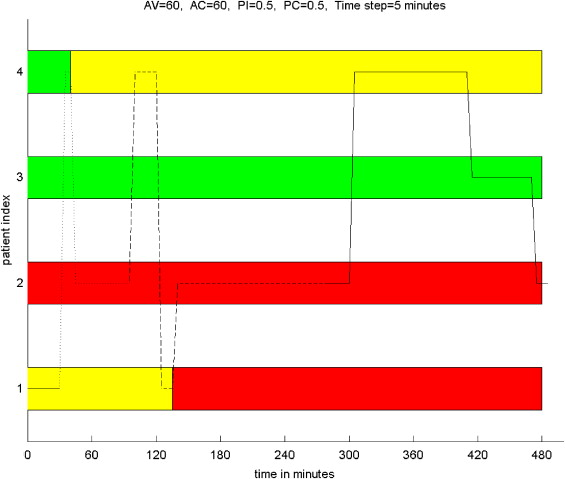
\includegraphics[width=0.8\textwidth]{FIGS/Dagata_etal_patients_profiles.jpg}
\end{center}
\vfill
\tiny Patient–HCW contact diagram for four patients and one HCW during one shift. Patient status: uninfected (green), infected with the non-resistant strain (yellow), infected with the resistant strain (red). HCW status: uncontaminated (plain), contaminated with the non-resistant strain (dotted), contaminated with the resistant strain (dashed)
\end{frame}


\begin{frame}
\begin{center}
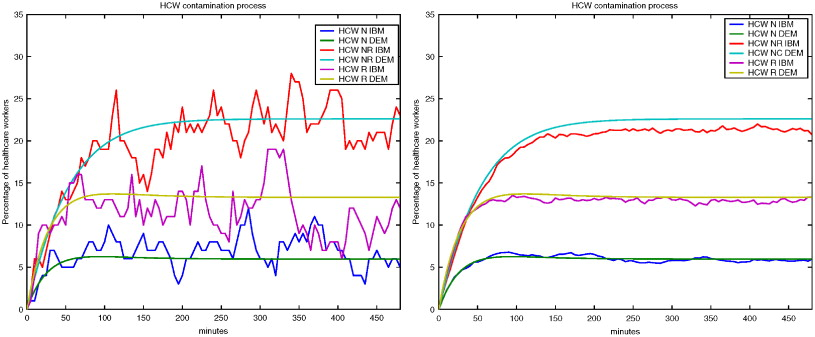
\includegraphics[width=\textwidth]{FIGS/Dagata_etal_comparisons.jpg}
\end{center}
\vfill
\tiny 
The left (respectively the right) figure corresponds to 1 trajectory (respectively the average over 80 trajectories) of the IBM during one shift, with no exit and admission of patients, and no changes in the infection status of patients
\end{frame}


\begin{frame}{Effectiveness of contact tracing in TB}
Tian, Osgood, Al-Azem \& Hoeppner. \href{https://doi-org.uml.idm.oclc.org/10.1177\%2F1090198113493910}{Evaluating the Effectiveness of Contact Tracing on Tuberculosis Outcomes in Saskatchewan Using Individual-Based Modeling}, Health Education \& Behavior (2013)
\end{frame}


\begin{frame}
\begin{center}
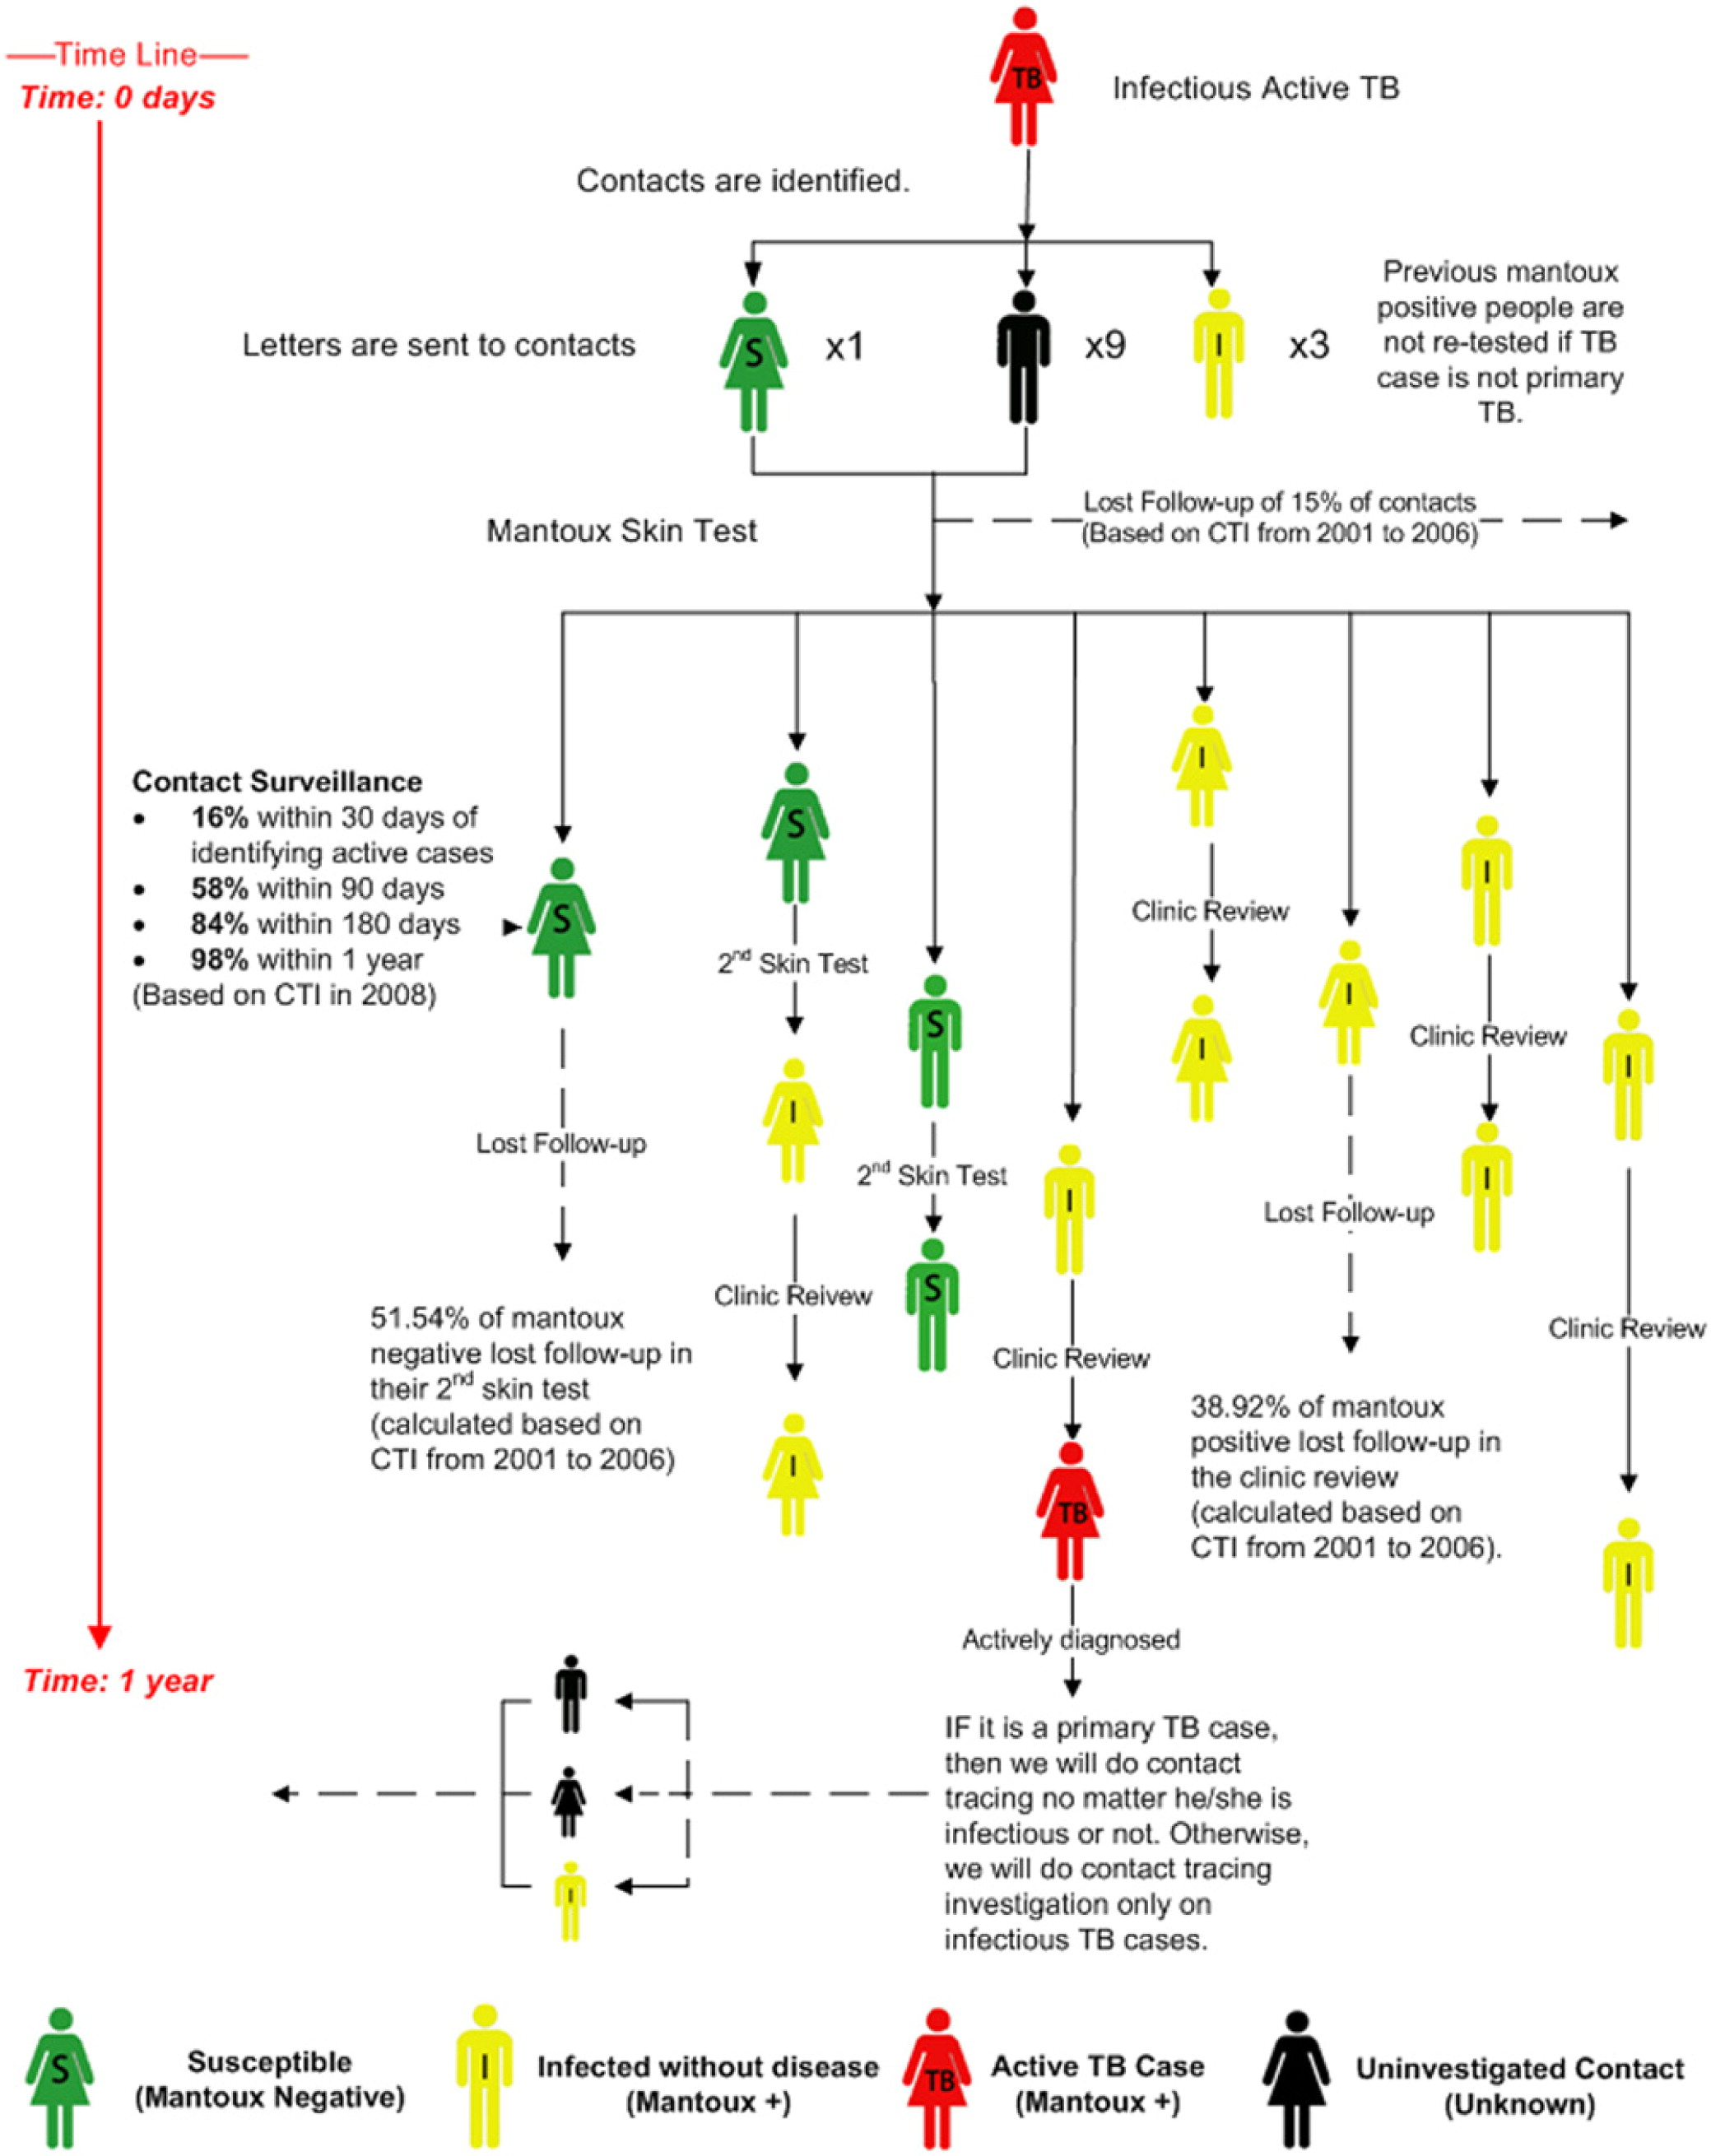
\includegraphics[width=\textwidth]{FIGS/TianOsgood_etal_TB_CT.jpeg}
\end{center}
\end{frame}

\begin{frame}
\begin{center}
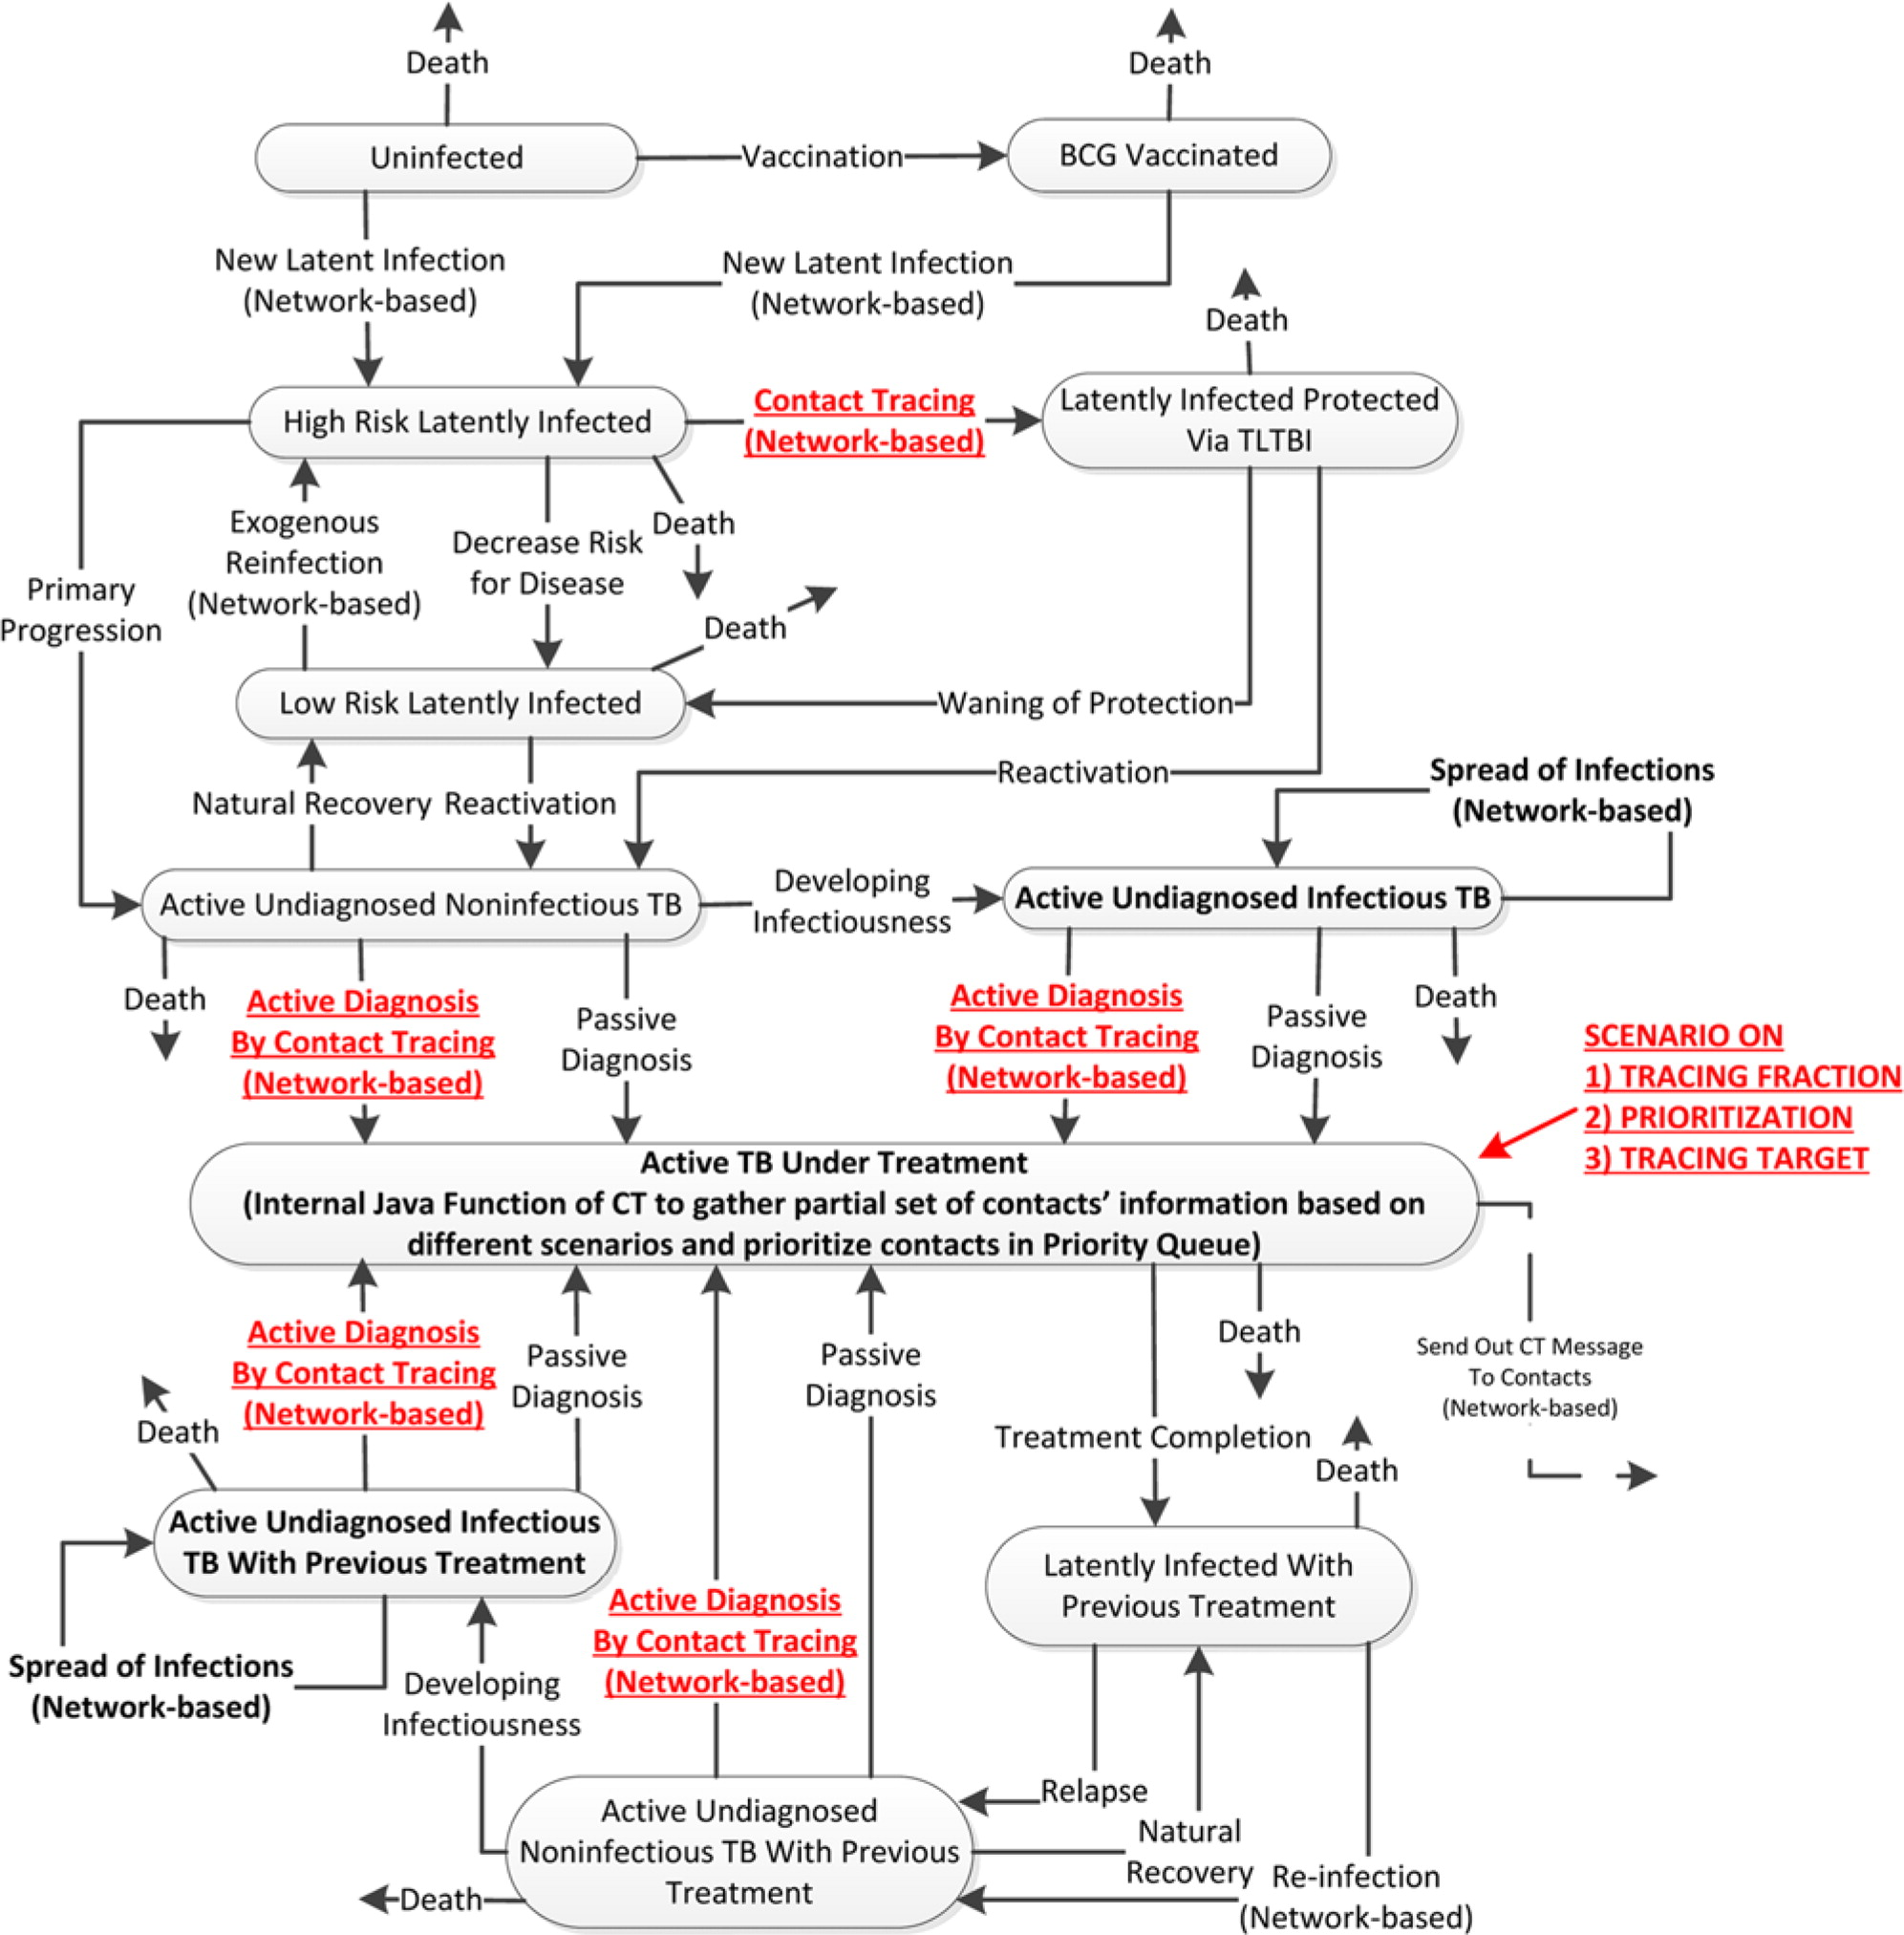
\includegraphics[width=\textwidth]{FIGS/TianOsgood_etal_state_flow_agent.jpeg}
\end{center}
\end{frame}


\begin{frame}
\begin{center}
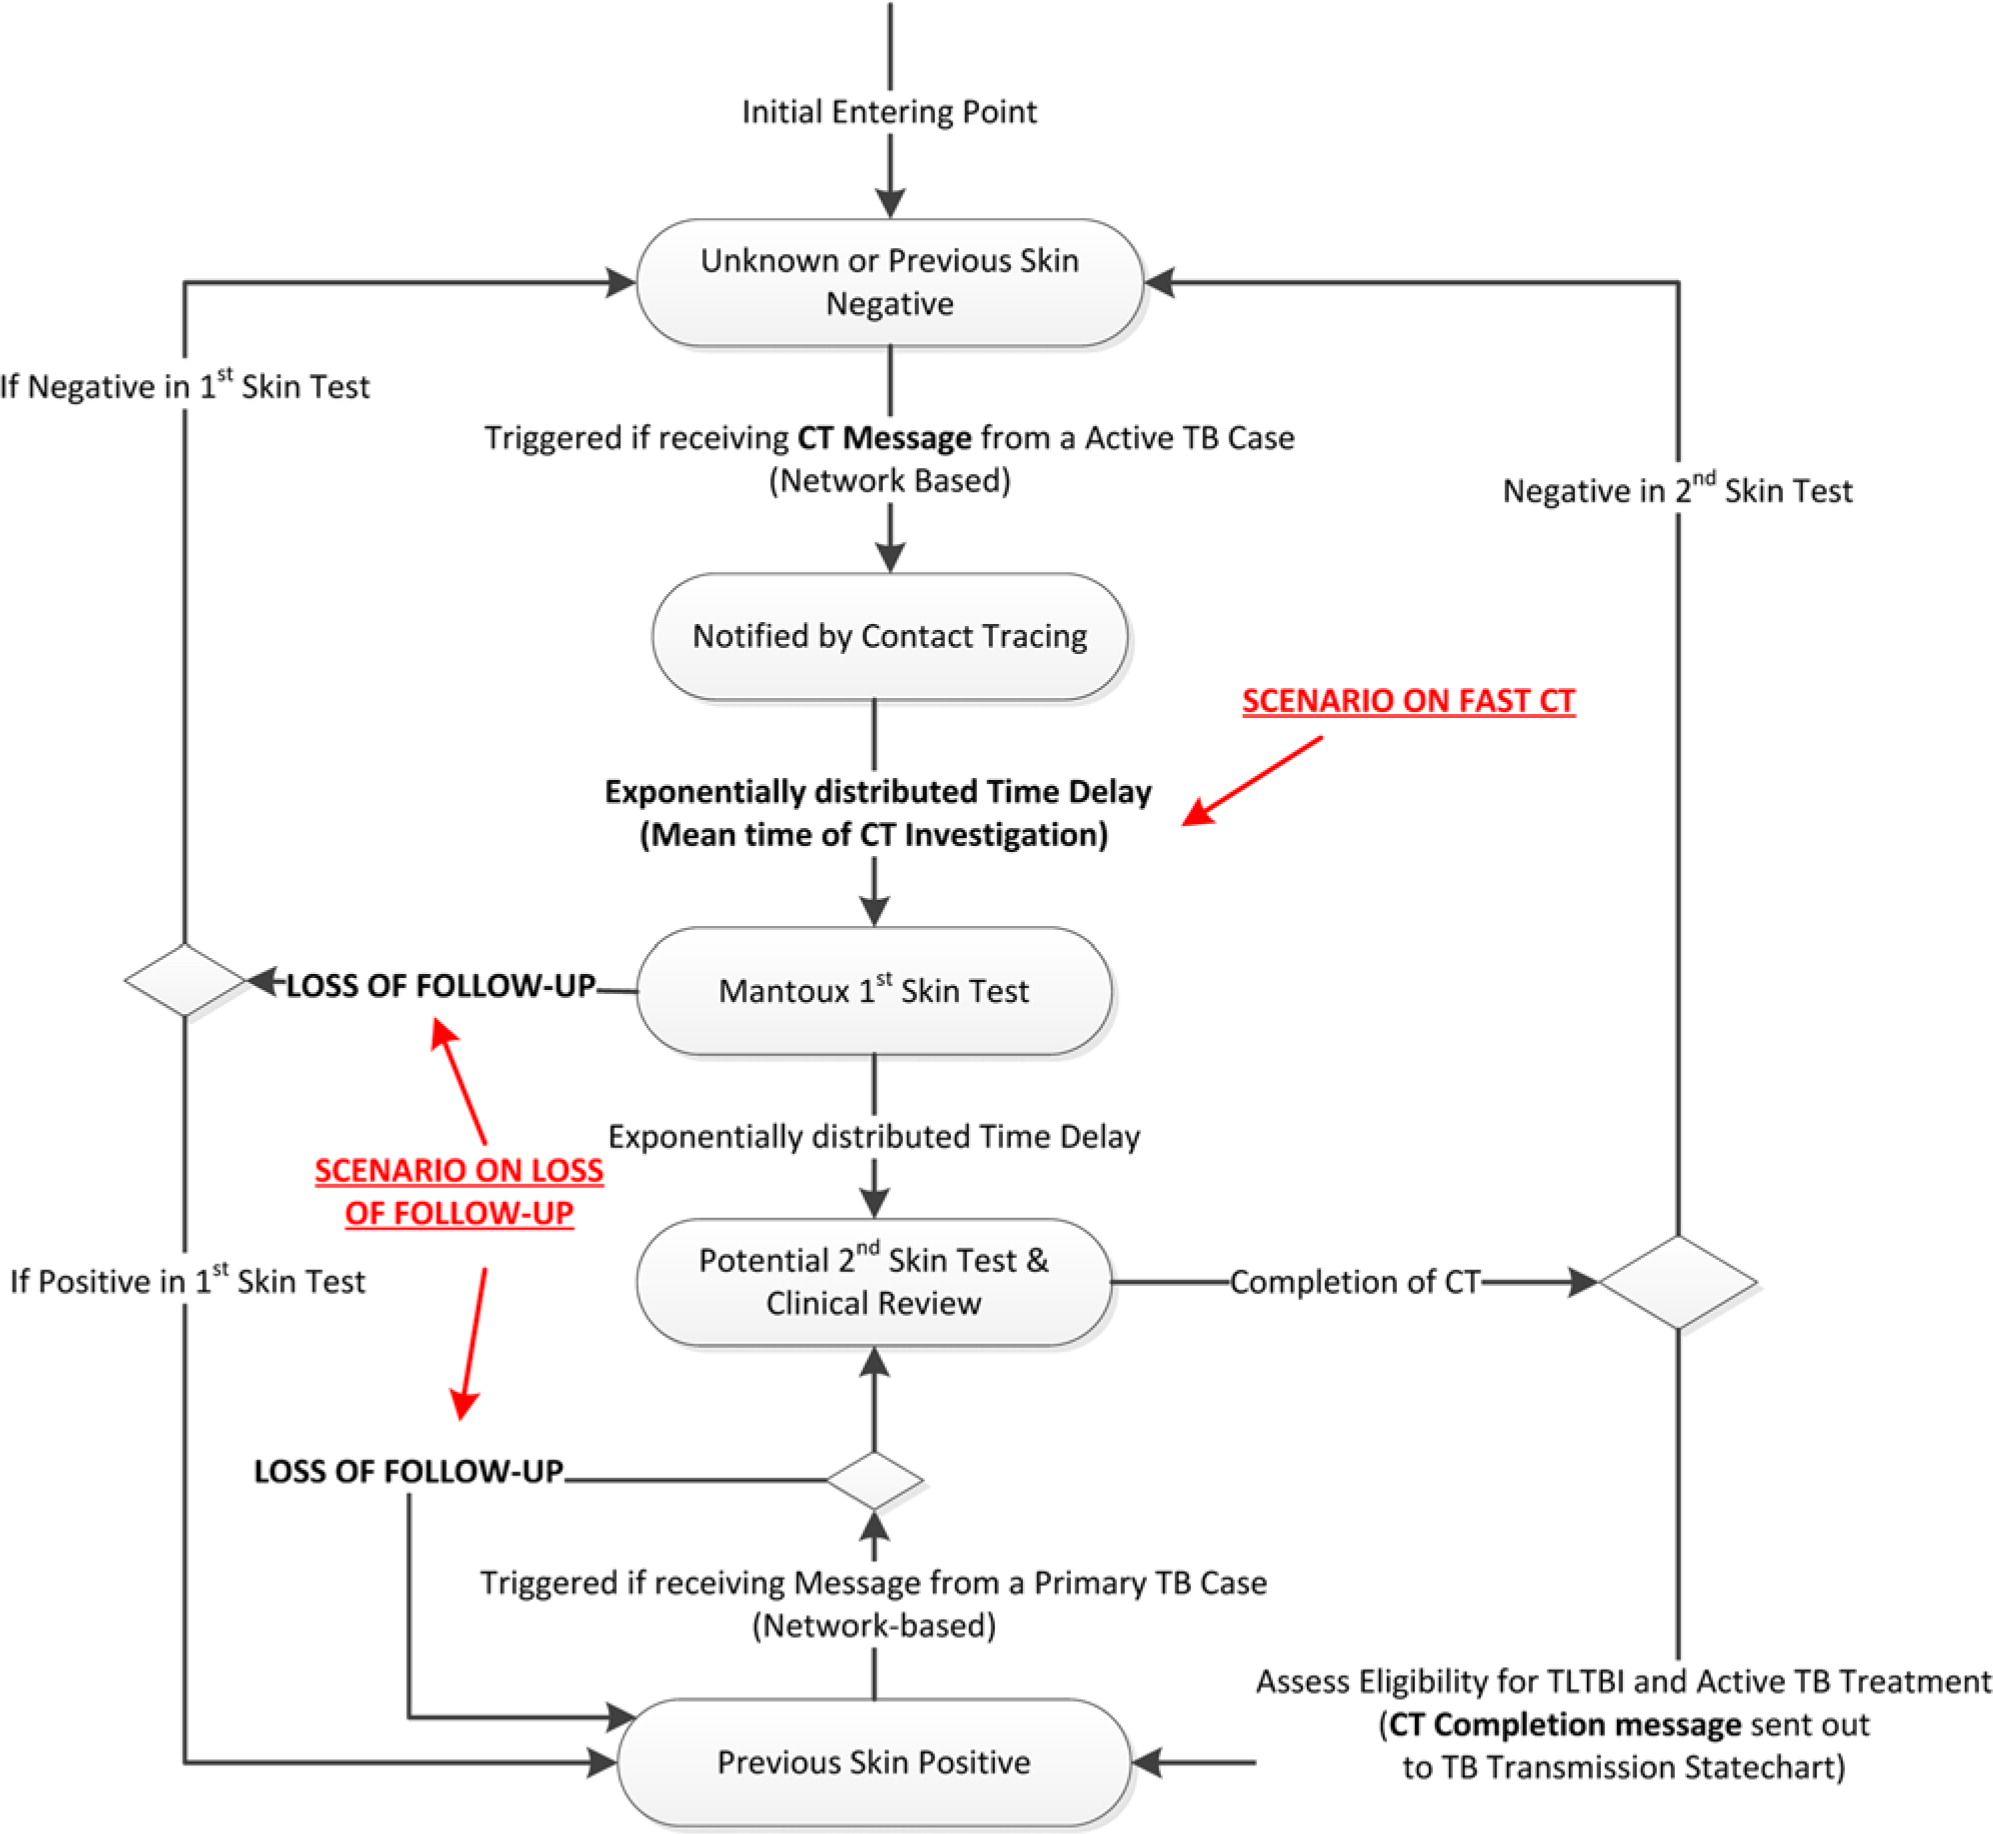
\includegraphics[width=\textwidth]{FIGS/TianOsgood_etal_model_CT.jpeg}
\end{center}
\end{frame}



\begin{frame}
They can then formulate scenarios
\begin{center}
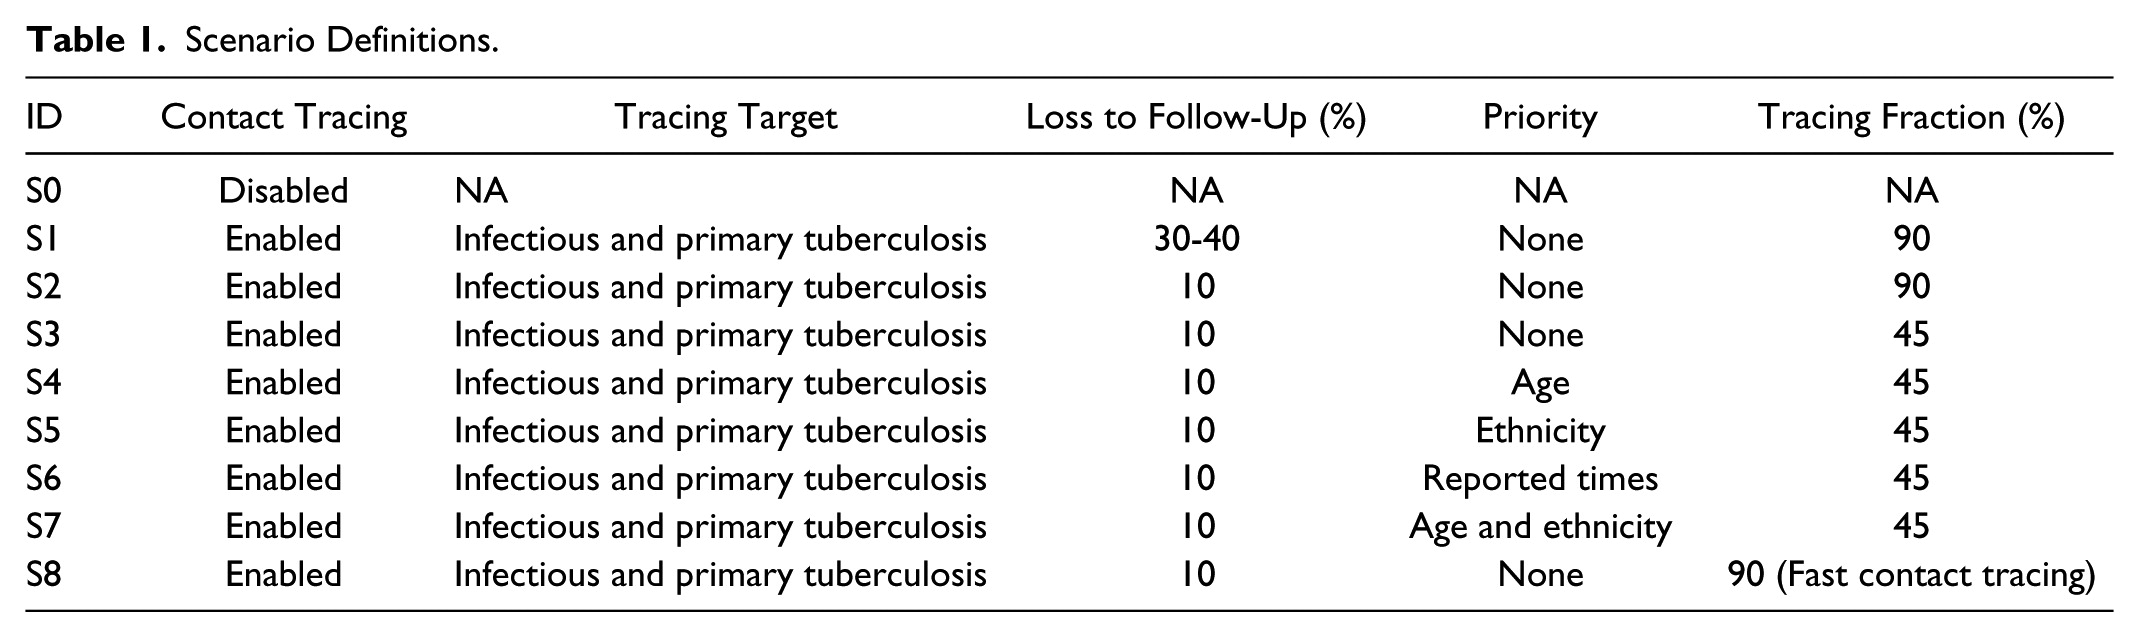
\includegraphics[width=\textwidth]{FIGS/TianOsgood_etal_scenarios.jpeg}
\end{center}
They then run these scenarios and compare results
\end{frame}


\begin{frame}
\begin{center}
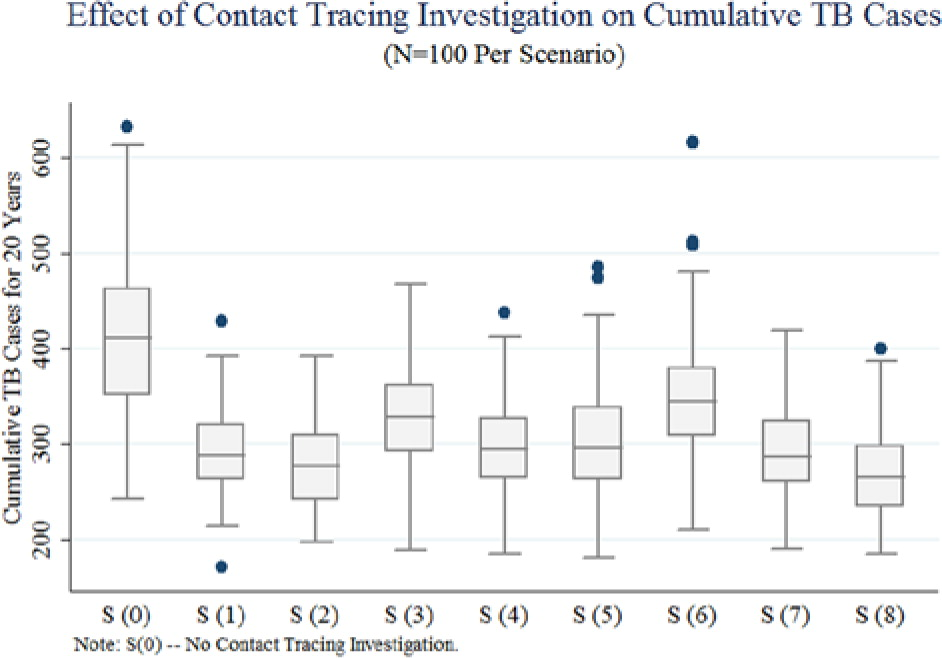
\includegraphics[width=\textwidth]{FIGS/TianOsgood_etal_scenario_results.jpeg}
\end{center}
\end{frame}


\begin{frame}{Contacts during Hajj}
Tofighi, Asgary, Tofighi, Najafabadi, Arino, Amiche, Rahman, McCarthy, Bragazzi, Thommes,  Coudeville, Grunnill, Bourouiba and Wu. \href{http://dx.doi.org/10.2139/ssrn.3678581}{Estimating Social Contacts in Mass Gatherings for Disease Outbreak Prevention and Management (Case of Hajj Pilgrimage)}, Tropical Diseases, Travel Medicine and Vaccines
\end{frame}

\begin{frame}{Contacts during Hajj}
In a mass gathering event like Hajj, lots of people come together originating from many countries
\vfill
So if propagation occurs during the event, this has the capacity to spread infection far and wide when individuals (pilgrims here) return home
\vfill
Contacts during part of the event are really specific in their configuration
\end{frame}


\begin{frame}{The setup}
Word of warning: I am quite fuzzy on the specifics :)
\vfill
Pilgrims enter Masjid al-Haram mosque through several gates
\vfill
Proceed to Mataaf (area around Kaaba), circle the Kaaba 7 times counterclockwise (process is the \emph{Tawaf})
\vfill
Then do seven trips between Safa and Marwah (process is the \emph{Sa'ee})
\end{frame}

\begin{frame}
\begin{center}
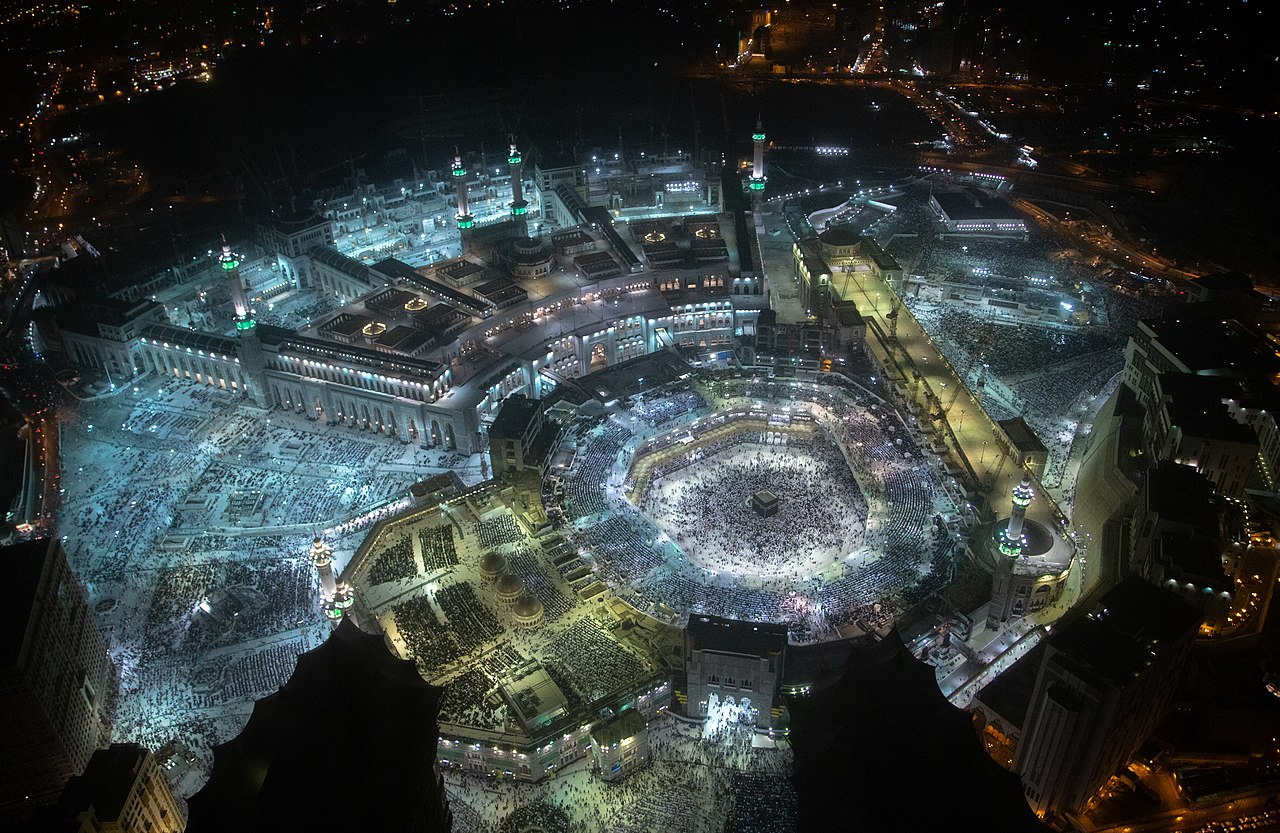
\includegraphics[width=\textwidth]{FIGS/Great_Mosque_of_Mecca.jpg}
\end{center}
\end{frame}

\begin{frame}
As you can gather from this:
\begin{itemize}
\item Typically high density crowds
\item Very specific mixing patterns
\end{itemize}
\vfill
Opportunities for transmission are very high
\vfill
However, control mechanisms are also available
\vfill
$\implies$ understanding contact patterns and frequency would help
\end{frame}


\begin{frame}
\begin{center}
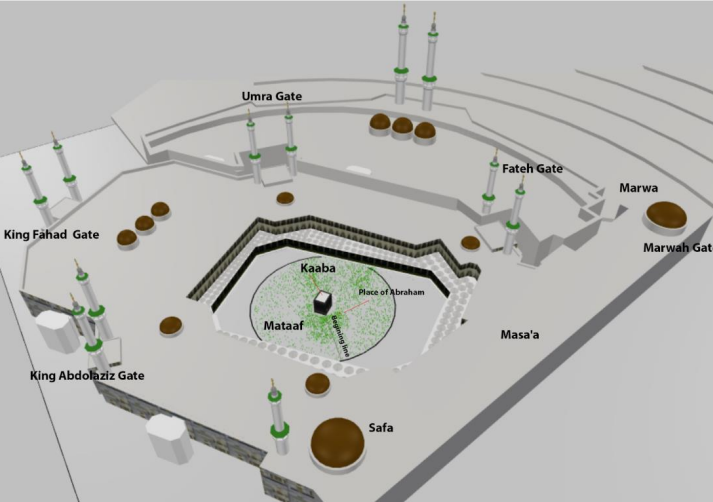
\includegraphics[width=\textwidth]{FIGS/ABM_Hajj_MAH_3Dmodel.png}
\end{center}
\end{frame}


\begin{frame}
\begin{center}
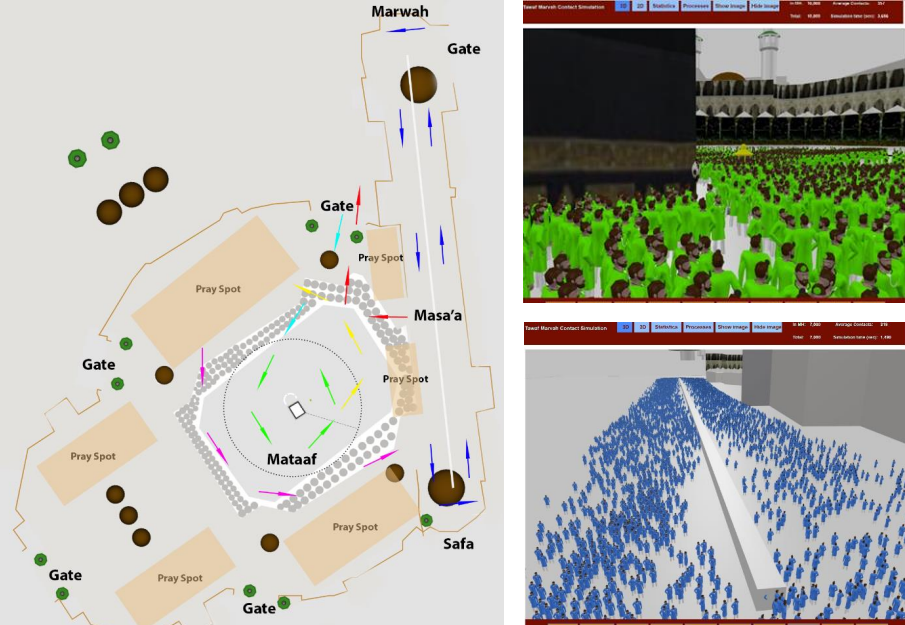
\includegraphics[width=\textwidth]{FIGS/ABM_Hajj_setup.png}
\end{center}
\end{frame}


\begin{frame}
\begin{center}
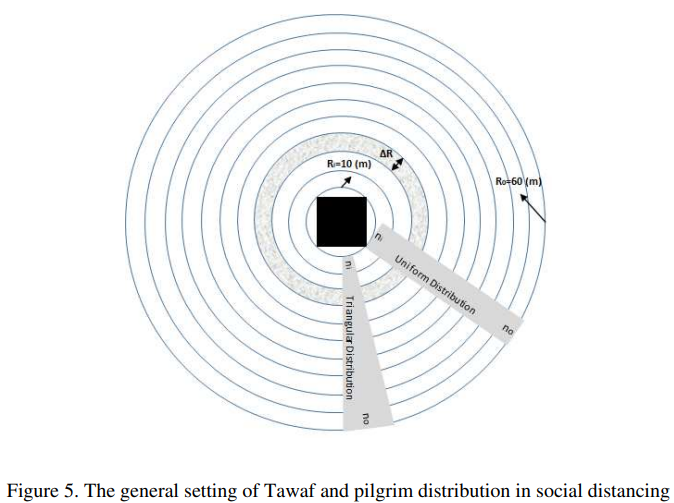
\includegraphics[width=\textwidth]{FIGS/ABM_Hajj_config_tawaf.png}
\end{center}
\end{frame}


%%%%%%%%%%%%%%%%%%%%%%%%%%%%%
%%%%%%%%%%%%%%%%%%%%%%%%%%%%%
%%%%%%%%%%%%%%%%%%%%%%%%%%%%%
%%%%%%%%%%%%%%%%%%%%%%%%%%%%%
\section{Network models}
%%%%%%%%%%%%%%%%%%%%%%%%%%%%%
%%%%%%%%%%%%%%%%%%%%%%%%%%%%%
\subsection{Why use network models}

\begin{frame}{Understand contact processes}
Classic models allow a certain degree of flexibility, for instance by using specific incidence functions or group models, but this remains limited and an approximation
\vfill
Like ABM, network models are used to make more realistic descriptions of the transmission of pathogens
\end{frame}


\begin{frame}{Human life is organised in networks}
Family
\vfill
Friends
\vfill
Workplace
\vfill
$\ldots$
\vfill
Social network theory has been used for years, e.g., in a professional context (e.g., how to fluidify interactions within a company)
\end{frame}



\subsection{Social networks}

\begin{frame}
Before considering epidemics in networks, it is useful to learn a few notions of social network theory, as this is very useful to understand networks
\vfill
Social network methods introduce measures that allow to evaluate some properties of graphs
\vfill
A network is a (mathematical) graph, oriented or not, in which edges/arcs represent connections (whathever they are) between individuals, who make up the vertices of the graph
\end{frame}



\begin{frame}{Context}
\bbullet $\mathcal{G}(\mathcal{V},\mathcal{E})$ an undirected graph
\vfill
\bbullet $\mathcal{D}(\mathcal{V},\mathcal{A})$ a digraph (directed graph)
\vfill
\bbullet $\mathcal{V}$ the set of vertices (or nodes)
\vfill
\bbullet $\mathcal{E}$ the set of edges (undirected case)
\vfill
\bbullet $\mathcal{A}$ the set of arcs (directed graph)
\end{frame}


\begin{frame}{Example of the global air transport network}
- Je vais illustrer avec des données du réseau de transport aérien mondial
- Données assez bonnes (très bonnes parfois), et un avantage flagrant:
  - Quand un avion part de quelque part et arrive ailleurs, c'est quelque chose d'assez .. déterministe
\end{frame}


\begin{frame}{The global air transportation network}
	\bigskip
	{\centering
		\hspace*{-\beamerleftmargin}
		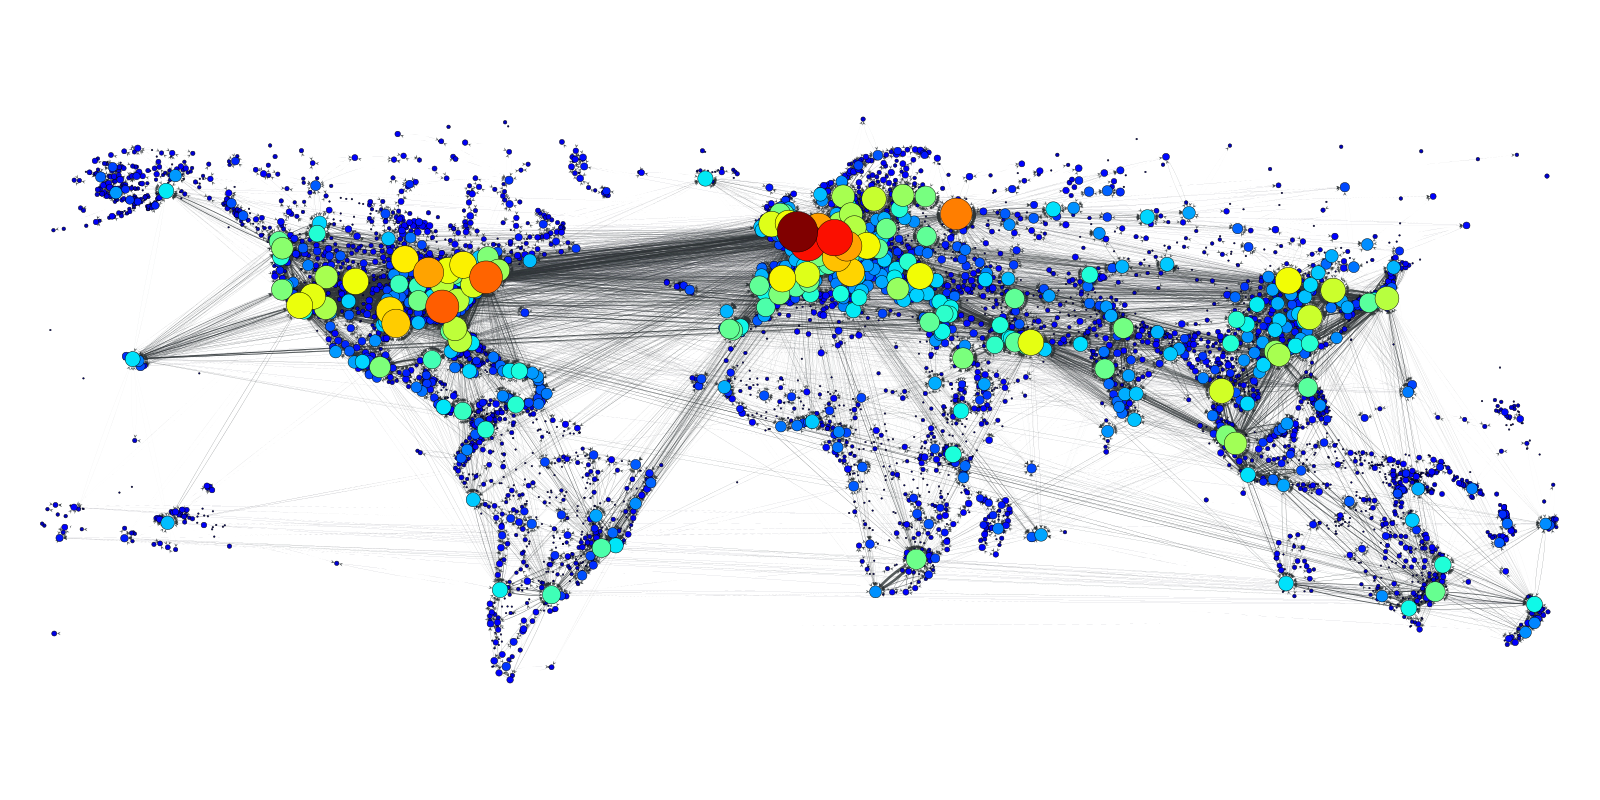
\includegraphics[width=\paperwidth]{FIGS/world_graph-degree}
	}
\end{frame}

\begin{frame}{Example of spread of p-H1N1}
	\bigskip
	{\centering
		\hspace*{-\beamerleftmargin}
		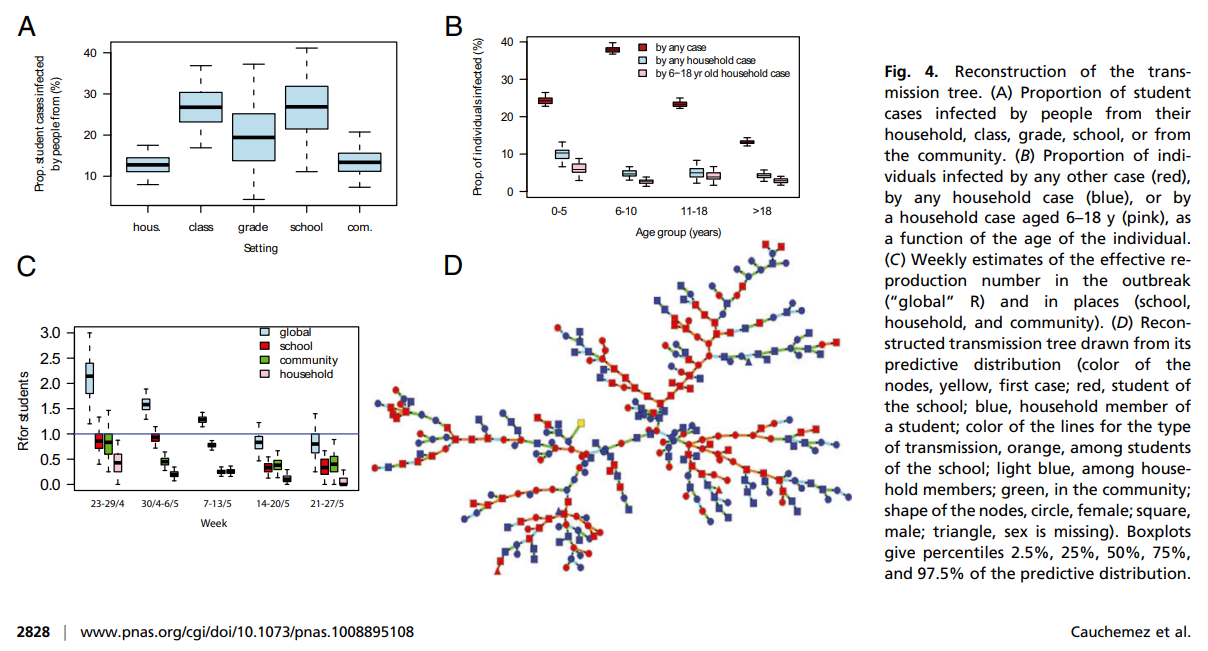
\includegraphics[width=\paperwidth]{FIGS/Cauchemez_etal_H1N1}
	}
	\vskip0pt plus 1filll
	\tiny
	Role of social networks in shaping disease transmission during a community outbreak of 2009 H1N1 pandemic influenza, Cauchemez \emph{et al}, PNAS \textbf{108}(7):2825-2830 (2011)
\end{frame}

\begin{frame}{Example of spread of MERS}
	\begin{minipage}{0.8\textwidth}
		\hspace*{-\beamerleftmargin}
		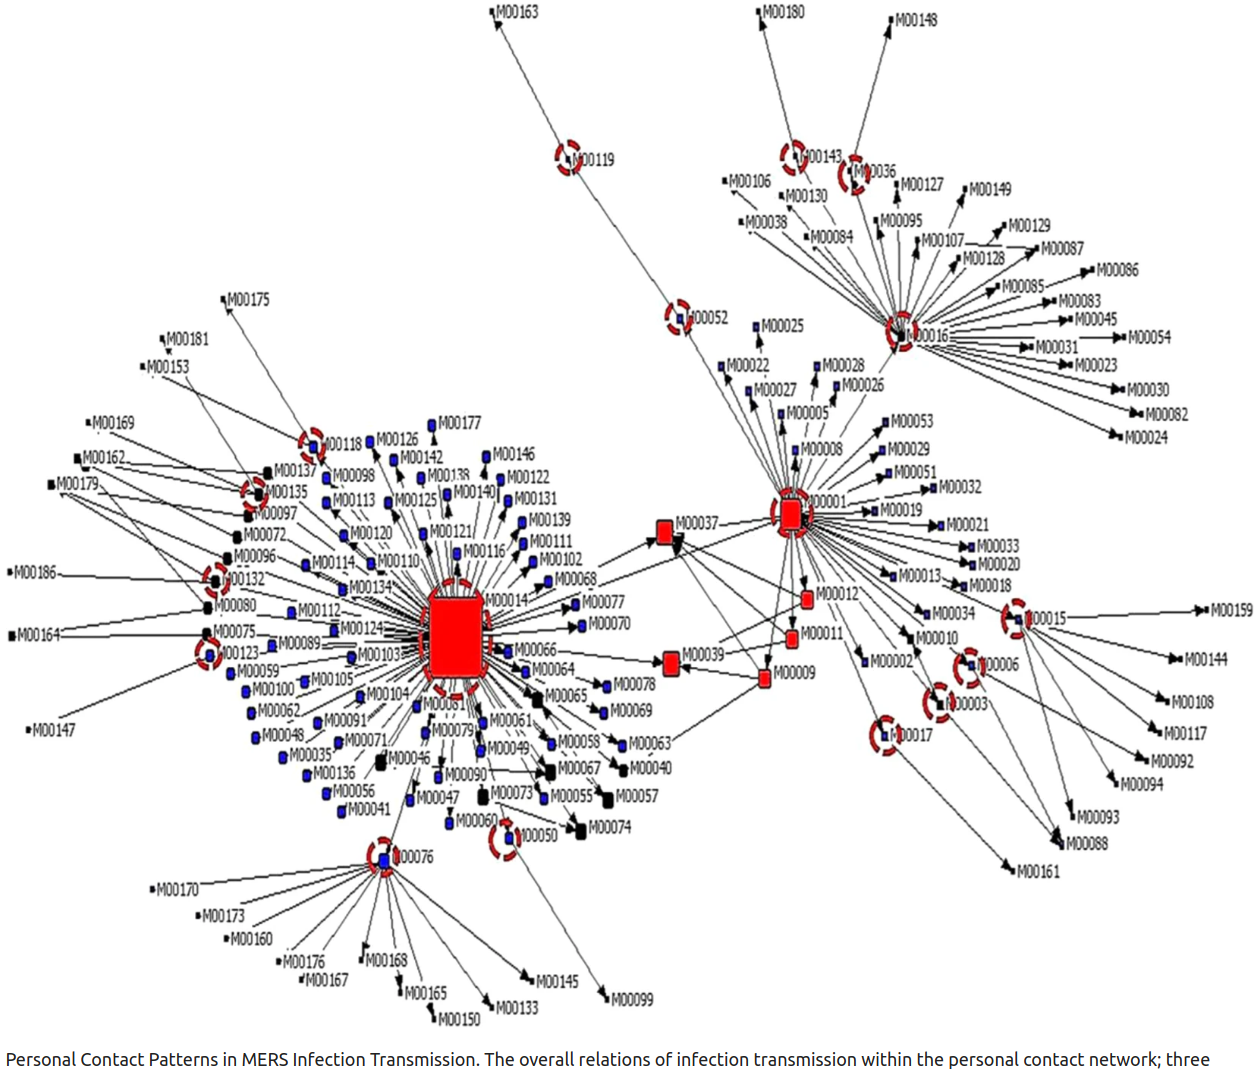
\includegraphics[height=\paperheight]{FIGS/YangJung2015SouthKoreaMERS}
	\end{minipage}
	\begin{minipage}{0.18\textwidth}
	\tiny
	Topological dynamics of the 2015 South Korea MERS-CoV spread-on-contact networks, Yang \& Jung, Scientific Reports \textbf{10}:4327 (2020)
	\end{minipage}
\end{frame}


\begin{frame}
	Some ``measures'' concern the vertices, others the graph as a whole
	
	In all that follows, unless otherwise indicated, $G=(X,A)$ is a digraph. If undirected, we write $G=(X,E)$.
\end{frame}

%%%%%%%%%%%%%%%%%%%%%
%%%%%%%%%%%%%%%%%%%%%
%%%%%%%%%%%%%%%%%%%%%
%%%%%%%%%%%%%%%%%%%%%
\subsection{Measures specific to vertices}


%%%%%%%%%%%%%%%%%%%%%
%%%%%%%%%%%%%%%%%%%%%
\subsubsection{Centre of a graph}

\begin{frame}{Geodesic distance}
\begin{definition}[Geodesic distance]
For $x,y\in X$, the \defword{geodesic distance} $d(x,y)$ is the length of the shortest path from $x$ to $y$, with $d(x,y)=\infty$ if no such path exists
\end{definition}
\end{frame}

\begin{frame}
	\begin{minipage}{0.5\textwidth}
	\begin{itemize}
	\item $d(x_1,x_2)=1$
	\item $d(x_1,x_3)=2$
	\item $\cdots$
	\end{itemize}
	\vfill
	\[
	\begin{pmatrix}
	0 & 1 & 2 & 2 & 4 & 3 \\
	1 & 0 & 1 & 1 & 3 & 2 \\
	3 & 4 & 0 & 5 & 2 & 1 \\
	4 & 5 & 1 & 0 & 3 & 2 \\
	1 & 2 & 3 & 3 & 0 & 4 \\
	2 & 3 & 4 & 4 & 1 & 0
	\end{pmatrix}		
	\]		
	\end{minipage}
	\begin{minipage}{0.49\textwidth}
		\def\skip{2.75cm}
		\begin{tikzpicture}[scale=0.75,auto,
			cloud/.style={minimum width={width("N-1")+2pt},
				draw, ellipse},
			connected/.style={dotted,-}]
			%% Vertices
			\node [cloud] at (0,0) (x1) {$x_1$};
			\node [cloud] at (1*\skip,1*\skip) (x2) {$x_2$};
			\node [cloud] at (2*\skip,1*\skip) (x3) {$x_3$};
			\node [cloud] at (1.5*\skip,0) (x4) {$x_4$};
			\node [cloud] at (3*\skip,0*\skip) (x5) {$x_5$};
			\node [cloud] at (3*\skip,1*\skip) (x6) {$x_6$};
			%% Arcs
			\path [line, thick,bend left] (x1) to (x2);
			\path [line, thick,bend left] (x2) to (x1);
			\path [line, thick, looseness=5] (x2) to (x2);
			\path [line, thick] (x2) to (x3);
			\path [line, thick] (x2) to (x4);
			\path [line, thick] (x4) to (x3);
			\path [line, thick, looseness=5, below] (x6) to (x6);
			\path [line, thick] (x6) to (x5);
			\path [line, thick] (x3) to (x6);
			\path [line, thick, bend left] (x5) to (x1);
			\end{tikzpicture}
\end{minipage}
\end{frame}

\begin{frame}
	\begin{minipage}{0.5\textwidth}
	\begin{itemize}
		\item $d(x_5,x_1)=\infty$
		\item $d(x_3,x_1)=\infty$
		\item $\cdots$
	\end{itemize}
	\vfill
	\[
	\begin{pmatrix}
		0 & 1 & 2 & 2 & 4 & 3 \\
		1 & 0 & 1 & 1 & 3 & 2 \\
		\infty & \infty & 0 & \infty & 2 & 1 \\
		\infty& \infty& 1 & 0 & 3 & 2 \\
		\infty& \infty & \infty & \infty & 0 & \infty \\
		\infty & \infty & \infty & \infty & 1 & 0
	\end{pmatrix}
	\]
	\end{minipage}
	\begin{minipage}{0.49\textwidth}
		\def\skip{2.75cm}
		\begin{tikzpicture}[scale=0.75,auto,
			cloud/.style={minimum width={width("N-1")+2pt},
				draw, ellipse},
			connected/.style={dotted,-}]
			%% Vertices
			\node [cloud] at (0,0) (x1) {$x_1$};
			\node [cloud] at (1*\skip,1*\skip) (x2) {$x_2$};
			\node [cloud] at (2*\skip,1*\skip) (x3) {$x_3$};
			\node [cloud] at (1.5*\skip,0) (x4) {$x_4$};
			\node [cloud] at (3*\skip,0*\skip) (x5) {$x_5$};
			\node [cloud] at (3*\skip,1*\skip) (x6) {$x_6$};
			%% Arcs
			\path [line, thick,bend left] (x1) to (x2);
			\path [line, thick,bend left] (x2) to (x1);
			\path [line, thick, looseness=5] (x2) to (x2);
			\path [line, thick] (x2) to (x3);
			\path [line, thick] (x2) to (x4);
			\path [line, thick] (x4) to (x3);
			\path [line, thick, looseness=5, below] (x6) to (x6);
			\path [line, thick] (x6) to (x5);
			\path [line, thick] (x3) to (x6);
			\end{tikzpicture}
	\end{minipage}
\end{frame}

\begin{frame}{Eccentricity}
\begin{definition}[Vertex eccentricity]
	The \textbf{eccentricity} $e(x)$ of vertex $x\in X$ is 
	\[
		e(x)=\max_{\stackrel{y\in X}{y\neq x}}d(x,y)
	\]
\end{definition}
\begin{minipage}{0.5\textwidth}
	\[
\begin{pmatrix}
	0 & 1 & 2 & 2 & \boldred{4} & 3 \\
	1 & 0 & 1 & 1 & \boldred{3} & 2 \\
	3 & 4 & 0 & \boldred{5} & 2 & 1 \\
	4 & \boldred{5} & 1 & 0 & 3 & 2 \\
	1 & 2 & 3 & 3 & 0 & \boldred{4} \\
	2 & 3 & \boldred{4} & \boldred{4} & 1 & 0
\end{pmatrix}		
\]
\end{minipage}
\begin{minipage}{0.49\textwidth}
	\def\skip{2.75cm}
	\begin{tikzpicture}[scale = 0.75,auto,
		cloud/.style={minimum width={width("N-1")+2pt},
			draw, ellipse},
		connected/.style={dotted,-}]
		%% Vertices
		\node [cloud] at (0,0) (x1) {$x_1$};
		\node [cloud] at (1*\skip,1*\skip) (x2) {$x_2$};
		\node [cloud] at (2*\skip,1*\skip) (x3) {$x_3$};
		\node [cloud] at (1.5*\skip,0) (x4) {$x_4$};
		\node [cloud] at (3*\skip,0*\skip) (x5) {$x_5$};
		\node [cloud] at (3*\skip,1*\skip) (x6) {$x_6$};
		%% Arcs
		\path [line, thick,bend left] (x1) to (x2);
		\path [line, thick,bend left] (x2) to (x1);
		\path [line, thick, looseness=5] (x2) to (x2);
		\path [line, thick] (x2) to (x3);
		\path [line, thick] (x2) to (x4);
		\path [line, thick] (x4) to (x3);
		\path [line, thick, looseness=5, below] (x6) to (x6);
		\path [line, thick] (x6) to (x5);
		\path [line, thick] (x3) to (x6);
		\path [line, thick, bend left] (x5) to (x1);
		\end{tikzpicture}
\end{minipage}
\end{frame}


\begin{frame}{Central points, radius and centre}
\begin{definition}[Central point]
	A \textbf{central point} of $G$ is a vertex $x_0$ with smallest eccentricity
\end{definition}
\vfill
\begin{definition}[Radius]
	The \textbf{radius} of $G$ is $\rho(G)=e(x_0)$, where $x_0$ is a centre of $G$
	In other words,
	\[
	\rho(G)=\min_{x\in X}e(x)
	\]
\end{definition}
\vfill
\begin{definition}[Centre]
The \textbf{centre} of $G$ is the set of vertices that are central points of $G$, i.e.,
\[
    \{x\in X: e(x)=\rho(G)\}
\]
\end{definition}
\end{frame}


\begin{frame}
	\begin{minipage}{0.5\textwidth}
	\[
\begin{pmatrix}
	0 & 1 & 2 & 2 & \boldred{4} & 3 \\
	\rowcolor{gray!95}
	1 & 0 & 1 & 1 & \boldred{3} & 2 \\
	3 & 4 & 0 & \boldred{5} & 2 & 1 \\
	4 & \boldred{5} & 1 & 0 & 3 & 2 \\
	1 & 2 & 3 & 3 & 0 & \boldred{4} \\
	2 & 3 & \boldred{4} & \boldred{4} & 1 & 0
\end{pmatrix}		
\]
%\vfill
Radius is 3, $x_2$ is a central point (the only one) and the centre is $\{x_2\}$
	\end{minipage}
	\begin{minipage}{0.49\textwidth}
		\def\skip{2.5cm}
		\begin{tikzpicture}[scale = 0.85,auto,
			cloud/.style={minimum width={width("N-1")+2pt},
				draw, ellipse},
			connected/.style={dotted,-}]
			%% Vertices
			\node [cloud] at (0,0) (x1) {$x_1$};
			\node [cloud, fill=gray!20] at (1*\skip,1*\skip) (x2) {$x_2$};
			\node [cloud] at (2*\skip,1*\skip) (x3) {$x_3$};
			\node [cloud] at (1.5*\skip,0) (x4) {$x_4$};
			\node [cloud] at (3*\skip,0*\skip) (x5) {$x_5$};
			\node [cloud] at (3*\skip,1*\skip) (x6) {$x_6$};
			%% Arcs
			\path [line, thick,bend left] (x1) to (x2);
			\path [line, thick,bend left] (x2) to (x1);
			\path [line, thick, looseness=5] (x2) to (x2);
			\path [line, thick] (x2) to (x3);
			\path [line, thick] (x2) to (x4);
			\path [line, thick] (x4) to (x3);
			\path [line, thick, looseness=5, below] (x6) to (x6);
			\path [line, thick] (x6) to (x5);
			\path [line, thick] (x3) to (x6);
			\path [line, thick, bend left] (x5) to (x1);
			\end{tikzpicture}
	\end{minipage}
\end{frame}


%%%%%%%%%%%%%%%%%%%%%
\subsubsection{Centrality -- Betweenness and closeness}
\begin{frame}{How \emph{central} is a vertex?}
	\emph{Centrality} tries to answer the question: what are the most influent vertices? 
	
	We have seen central vertices and vertices on the periphery, let us consider two other measures of centrality
	\begin{itemize}
			\item Betweenness centrality
			\item Closeness centrality
	\end{itemize}
	Many other forms (we will come back to this, e.g., degree centrality)
\end{frame}

\begin{frame}{Betweenness}
\begin{definition}[Betweenness]
	$G=(X,U)$ a graph, $x\in X$. The \textbf{betweenness} of $v$ is
	\[
	b_\D(v)= \sum_{s\neq t\neq v  \in X} \frac{\sigma_{st}(v)}{\sigma_{st}}
	\]
	where
	\begin{itemize}
	\item $\sigma_{st}$ number of shortest geodesic paths from $s$ to $t$
	\item $\sigma_{st}(v)$ number of shortest geodesic paths from $s$ to $t$ through $v$
	\end{itemize}		
\end{definition}
\vfill
In other words
\begin{itemize}
	\item For each pair of vertices $(s,t)$, compute the shortest paths between them
	\item For each pair of vertices $(s,t)$, determine the fraction of shortest paths that pass through vertex $v$
	\item Sum this fraction over all pairs of vertices $(s,t)$
\end{itemize}
\end{frame}

\begin{frame}{Normalising betweenness}
	Betweenness may be normalized by dividing through the number of pairs of vertices not including $v$:
	\begin{itemize}
		\item for directed graphs, $(n-1)(n-2)$
		\item for undirected graphs, $(n-1)(n-2)/2$
	\end{itemize}
\end{frame}


\begin{frame}{Example of betweenness}
	\begin{minipage}{0.39\textwidth}
		{\tt distances(G, mode="out")}
		\[
			\begin{pmatrix}
				0 & 1 & 2 & 2 & 4 & 3 \\
				1 & 0 & 1 & 1 & 3 & 2 \\
				3 & 4 & 0 & 5 & 2 & 1 \\
				4 & 5 & 1 & 0 & 3 & 2 \\
				1 & 2 & 3 & 3 & 0 & 4 \\
				2 & 3 & 4 & 4 & 1 & 0
			\end{pmatrix}
		\]
		\end{minipage}
	\begin{minipage}{0.6\textwidth}
		\def\skip{2.75cm}
		\begin{tikzpicture}[scale = 0.85,
			every node/.style={transform shape},
			auto,
			cloud/.style={minimum width={width("N-1")+2pt},
				draw, ellipse},
			connected/.style={dotted,-}]
			%% Vertices
			\node [cloud] at (0,0) (x1) {$x_1$};
			\node [cloud] at (1*\skip,1*\skip) (x2) {$x_2$};
			\node [cloud] at (2*\skip,1*\skip) (x3) {$x_3$};
			\node [cloud] at (1.5*\skip,0) (x4) {$x_4$};
			\node [cloud] at (3*\skip,0*\skip) (x5) {$x_5$};
			\node [cloud] at (3*\skip,1*\skip) (x6) {$x_6$};
			%% Arcs
			\path [line, thick,bend left] (x1) to (x2);
			\path [line, thick,bend left] (x2) to (x1);
			\path [line, thick] (x2) to (x3);
			\path [line, thick] (x2) to (x4);
			\path [line, thick] (x4) to (x3);
			\path [line, thick] (x6) to (x5);
			\path [line, thick] (x3) to (x6);
			\path [line, thick, bend left] (x5) to (x1);
			\path [line, thick, looseness=5] (x2) to (x2);
			\path [line, thick, looseness=5, below] (x6) to (x6);
		\end{tikzpicture}
	\end{minipage}
\end{frame}


\begin{frame}{Number of shortest paths}
	Recall we found 
	{\tt distances(G, mode="out")}
	\[
		\mathcal{D} =
		\begin{pmatrix}
			0 & 1 & 2 & 2 & 4 & 3 \\
			1 & 0 & 1 & 1 & 3 & 2 \\
			3 & 4 & 0 & 5 & 2 & 1 \\
			4 & 5 & 1 & 0 & 3 & 2 \\
			1 & 2 & 3 & 3 & 0 & 4 \\
			2 & 3 & 4 & 4 & 1 & 0
		\end{pmatrix}
	\]
	\vfill
	To find the number of shortest paths between pairs of vertices, we can use powers of the adjacency matrix
	\vfill
	Write $\mathcal{D}=[d_{ij}]$, for a given $(i,j)$ ($i\neq j$), if $d_{ij}=k$, then pick the $(i,j)$ in $A^k$
\end{frame}

\begin{frame}
	We find
	\[
		\begin{pmatrix}
			0 & 1 & 1 & 1 & 1 & 1 \\
			1 & 0 & 1 & 1 & 1 & 1 \\
			1 & 1 & 0 & 1 & 1 & 1 \\
			1 & 1 & 1 & 0 & 1 & 1 \\
			1 & 1 & 1 & 1 & 0 & 1 \\
			1 & 1 & 1 & 1 & 1 & 0
		\end{pmatrix}
	\]
	\vfill
	Recall that betweenness of $v$ is
	\[
		b_\D(v)= \sum_{s\neq t\neq v  \in X} \frac{\sigma_{st}(v)}{\sigma_{st}}
	\]
	\vfill
	$\sigma_{st}$ (\# shortest paths from $s$ to $t$) is found in the matrix above
	\vfill
	What about $\sigma_{st}(v)$, \# of those shortest paths that go through $v$?
	\vfill
	We can use {\tt all\_shortest\_paths(G, from = s, to = t, mode = "out")}
\end{frame}


\begin{frame}{Example of betweenness}
	\begin{minipage}{0.35\textwidth}
		{\tt betweenness(G, directed = FALSE, normalized = TRUE)}

		Values shown in the vertices.
	\end{minipage}
	\begin{minipage}{0.6\textwidth}
		\def\skip{2.75cm}
		\begin{tikzpicture}[scale = 0.85,
			every node/.style={transform shape},
			auto,
			cloud/.style={minimum width={width("N-1")+2pt},
				draw, ellipse},
			connected/.style={dotted,-}]
			%% Vertices
			\node [cloud] at (0,0) (x1) {$0.5$};
			\node [cloud] at (1*\skip,1*\skip) (x2) {$0.5$};
			\node [cloud] at (2*\skip,1*\skip) (x3) {$0.45$};
			\node [cloud] at (1.5*\skip,0) (x4) {$0$};
			\node [cloud] at (3*\skip,0*\skip) (x5) {$0.45$};
			\node [cloud] at (3*\skip,1*\skip) (x6) {$0.45$};
			%% Arcs
			\path [line, thick,bend left] (x1) to (x2);
			\path [line, thick,bend left] (x2) to (x1);
			\path [line, thick] (x2) to (x3);
			\path [line, thick] (x2) to (x4);
			\path [line, thick] (x4) to (x3);
			\path [line, thick] (x6) to (x5);
			\path [line, thick] (x3) to (x6);
			\path [line, thick, bend left] (x5) to (x1);
			\path [line, thick, looseness=5] (x2) to (x2);
			\path [line, thick, looseness=5, below] (x6) to (x6);
		\end{tikzpicture}
	\end{minipage}
\end{frame}


\begin{frame}{Closeness}
	\begin{definition}
		$G=(X,U)$, $v\in X$. The \textbf{closeness} of $v$ is
		\[
		c_\D(v)=\frac{1}{n-1}\displaystyle \sum_{t\in X\setminus\{v\}}d_\D(v,t)
		\]
		i.e., mean geodesic distance between a vertex $v$ and all other vertices it has access to
		\vskip1cm 
		Another definition is
		\[
		c_\D(v)=\frac{1}{\displaystyle\sum_{t \in X\setminus\{v\}}d_\D(v,t)}
		\]				
	\end{definition}
\end{frame}

\begin{frame}{Example of (out) closeness}
	\vfill
	{\tt closeness(G, normalized = TRUE, mode=``out'')}
	\vfill
	\begin{center}
		\def\skip{2.75cm}
		\begin{tikzpicture}[scale = 0.85,
			every node/.style={transform shape},
			auto,
			cloud/.style={minimum width={width("N-1")+2pt},
				draw, ellipse},
			connected/.style={dotted,-}]
			%% Vertices
			\node [cloud] at (0,0) (x1) {$0.417$};
			\node [cloud] at (1*\skip,1*\skip) (x2) {$0.625$};
			\node [cloud] at (2*\skip,1*\skip) (x3) {$0.333$};
			\node [cloud] at (1.5*\skip,0) (x4) {$0.333$};
			\node [cloud] at (3*\skip,0*\skip) (x5) {$0.385$};
			\node [cloud] at (3*\skip,1*\skip) (x6) {$0.357$};
			%% Arcs
			\path [line, thick,bend left] (x1) to (x2);
			\path [line, thick,bend left] (x2) to (x1);
			\path [line, thick] (x2) to (x3);
			\path [line, thick] (x2) to (x4);
			\path [line, thick] (x4) to (x3);
			\path [line, thick] (x6) to (x5);
			\path [line, thick] (x3) to (x6);
			\path [line, thick, bend left] (x5) to (x1);
			\path [line, thick, looseness=5] (x2) to (x2);
			\path [line, thick, looseness=5, below] (x6) to (x6);
		\end{tikzpicture}
	\end{center}
\end{frame}

%%%%%%%%%%%%%%%%%%%%%
\subsubsection{Periphery of a graph}
\begin{frame}{Diametre and periphery of a graph}
\begin{definition}[Diametre of a graph]
The \textbf{diametre} of $G$ is 
\[
	\delta(G) = \max_{\stackrel{x,y\in X}{x\neq y}}d(x,y)
\]
or, in other words,
\[
	\delta(G)= \max_{x\in X}e(x)
\]
\end{definition}
\vfill
$\delta(G)<\infty$ $\iff$ $G$ strongly connected
\vfill
\begin{definition}[Periphery]
    The \textbf{periphery} of a graph is the set of vertices whose eccentricity achieves the diametre, i.e.,
    \[
        \{x\in X:e(x)=\delta(G)\}
    \]
\end{definition}
\end{frame}


\begin{frame}
		\begin{minipage}{0.5\textwidth}
	\[
\begin{pmatrix}
	0 & 1 & 2 & 2 & \boldred{4} & 3 \\
	1 & 0 & 1 & 1 & \boldred{3} & 2 \\
	\rowcolor{gray!95}
	3 & 4 & 0 & \boldred{5} & 2 & 1 \\
	\rowcolor{gray!95}
	4 & \boldred{5} & 1 & 0 & 3 & 2 \\
	1 & 2 & 3 & 3 & 0 & \boldred{4} \\
	2 & 3 & \boldred{4} & \boldred{4} & 1 & 0
\end{pmatrix}		
\]
Diametre is 5 and the periphery is $\{x_3,x_4\}$
	\end{minipage}
	\begin{minipage}{0.49\textwidth}
		\def\skip{2.5cm}
		\begin{tikzpicture}[scale = 0.85,auto,
			cloud/.style={minimum width={width("N-1")+2pt},
				draw, ellipse},
			connected/.style={dotted,-}]
			%% Vertices
			\node [cloud] at (0,0) (x1) {$x_1$};
			\node [cloud] at (1*\skip,1*\skip) (x2) {$x_2$};
			\node [cloud, fill=gray!20] at (2*\skip,1*\skip) (x3) {$x_3$};
			\node [cloud, fill=gray!20] at (1.5*\skip,0) (x4) {$x_4$};
			\node [cloud] at (3*\skip,0*\skip) (x5) {$x_5$};
			\node [cloud] at (3*\skip,1*\skip) (x6) {$x_6$};
			%% Arcs
			\path [line, thick,bend left] (x1) to (x2);
			\path [line, thick,bend left] (x2) to (x1);
			\path [line, thick, looseness=5] (x2) to (x2);
			\path [line, thick] (x2) to (x3);
			\path [line, thick] (x2) to (x4);
			\path [line, thick] (x4) to (x3);
			\path [line, thick, looseness=5, below] (x6) to (x6);
			\path [line, thick] (x6) to (x5);
			\path [line, thick] (x3) to (x6);
			\path [line, thick, bend left] (x5) to (x1);
			\end{tikzpicture}
		\end{minipage}	
	\begin{definition}[{Antipodal vertices}]
			A pair of vertices $x$ and $y$ are \defword{antipodal} if they satisfy $d(x,y)=\delta(G)$.
	\end{definition}
\end{frame}


%%%%%%%%%%%%%%%%%%%%%
\subsubsection{Degree distribution}

\begin{frame}{Degree distribution}
	\begin{definition}[Arc incident to a vertex]
		If a vertex $x$ is the initial endpoint of an arc $u$, which is not a loop, the arc $u$ is \textbf{incident out of vertex} $x$ 
		\vskip0.2cm
		The number of arcs incident out of $x$ plus the number of loops attached to $x$ is denoted $d_G^+(x)$ and is the \textbf{outer demi-degree} of $x$
		\vskip0.2cm
		An arc \textbf{incident into vertex} $x$ and the \textbf{inner demi-degree} $d_G^-(x)$ are defined similarly
		\end{definition}
		\vfill
		\begin{definition}[Degree]
		The \textbf{degree} of vertex $x$ is the number of arcs with $x$ as an endpoint, each loop being counted twice. The degree of $x$ is denoted $d_G(x)=d_G^+(x)+d_G^-(x)$
		\vskip0.2cm
		If each vertex has the same degree, the graph is \textbf{regular}
	\end{definition}
\end{frame}

\begin{frame}
	\begin{definition}[{Isolated vertex}]
	A vertex of degree $0$ is \textbf{isolated}.
	\end{definition}
	\begin{definition}[{Average degree of $G$}]
	$d(G)=\frac{1}{|V|}\sum_{v\in V}deg_G(v)$.
	\end{definition}
	\begin{definition}[{Minimum degree of $G$}]
	$\delta(G)=\min \{deg_G(v)|v\in V\}$.
	\end{definition}
	\begin{definition}[{Maximum degree of $G$}]
	$\Delta(G)=\max \{deg_G(v)|v\in V\}$.
	\end{definition}
\end{frame}


\begin{frame}{Degrees in an undirected graph}
	\begin{minipage}{0.65\textwidth}
		\def\skip{2.75cm}
		\begin{tikzpicture}[scale=0.75,auto,
			cloud/.style={minimum width={width("N-1")+2pt},
				draw, ellipse},
			connected/.style={dotted,-}]
			%% Vertices
			\node [cloud] at (0,0) (x1) {$2$};
			\node [cloud] at (1*\skip,1*\skip) (x2) {$3$};
			\node [cloud] at (2*\skip,1*\skip) (x3) {$3$};
			\node [cloud] at (1.5*\skip,0) (x4) {$2$};
			\node [cloud] at (3*\skip,0*\skip) (x5) {$2$};
			\node [cloud] at (3*\skip,1*\skip) (x6) {$2$};
			%% Arcs
			\draw [thick] (x1) --  (x2);
			\draw [thick] (x2) --  (x3);
			\draw [thick] (x2) --  (x4);
			\draw [thick] (x3) --  (x6);
			\draw [thick] (x4) --  (x3);
			\draw [thick] (x6) --  (x5);
			\draw (x5) to[thick, out=-150, in=-30] (x1);
			\end{tikzpicture}
	\end{minipage}
	\begin{minipage}{0.3\textwidth}
		Here, vertices are labelled using the degree
	\end{minipage}
\end{frame}


\begin{frame}{Degrees in a directed graph}
	\begin{minipage}{0.45\textwidth}
		\def\skip{2.75cm}
		\begin{tikzpicture}[scale = 0.65, 
			every node/.style={transform shape},
			auto,
			cloud/.style={minimum width={width("N-1")+2pt},
				draw, ellipse},
			connected/.style={dotted,-}]
			%% Vertices
			\node [cloud] at (0,0) (x1) {$\begin{matrix}d^+=1\\ d^-=2\end{matrix}$};
			\node [cloud] at (1*\skip,1*\skip) (x2) {$\begin{matrix}d^+=3\\ d^-=1\end{matrix}$};
			\node [cloud] at (2*\skip,1*\skip) (x3) {$\begin{matrix}d^+=1\\ d^-=2\end{matrix}$};
			\node [cloud] at (1.5*\skip,0) (x4) {$\begin{matrix}d^+=1\\ d^-=1\end{matrix}$};
			\node [cloud] at (3*\skip,0*\skip) (x5) {$\begin{matrix}d^+=1\\ d^-=1\end{matrix}$};
			\node [cloud] at (3*\skip,1*\skip) (x6) {$\begin{matrix}d^+=1\\ d^-=1\end{matrix}$};
			%% Arcs
			\path [line, thick,bend left] (x1) to (x2);
			\path [line, thick,bend left] (x2) to (x1);
			\path [line, thick] (x2) to (x3);
			\path [line, thick] (x2) to (x4);
			\path [line, thick] (x4) to (x3);
			\path [line, thick] (x6) to (x5);
			\path [line, thick] (x3) to (x6);
			\path [line, thick, bend left] (x5) to (x1);
			\end{tikzpicture}
	\end{minipage}
	\quad
	\begin{minipage}{0.45\textwidth}
		\def\skip{2.75cm}
		\begin{tikzpicture}[scale = 0.65, 
			every node/.style={transform shape},
			auto,
			cloud/.style={minimum width={width("N-1")+2pt},
				draw, ellipse},
			connected/.style={dotted,-}]
			%% Vertices
			\node [cloud] at (0,0) (x1) {$\begin{matrix}d^+=1\\ d^-=2\end{matrix}$};
			\node [cloud] at (1*\skip,1*\skip) (x2) {$\begin{matrix}d^+=4\\ d^-=2\end{matrix}$};
			\node [cloud] at (2*\skip,1*\skip) (x3) {$\begin{matrix}d^+=1\\ d^-=2\end{matrix}$};
			\node [cloud] at (1.5*\skip,0) (x4) {$\begin{matrix}d^+=1\\ d^-=1\end{matrix}$};
			\node [cloud] at (3*\skip,0*\skip) (x5) {$\begin{matrix}d^+=1\\ d^-=1\end{matrix}$};
			\node [cloud] at (3*\skip,1*\skip) (x6) {$\begin{matrix}d^+=2\\ d^-=2\end{matrix}$};
			%% Arcs
			\path [line, thick,bend left] (x1) to (x2);
			\path [line, thick,bend left] (x2) to (x1);
			\path [line, thick] (x2) to (x3);
			\path [line, thick] (x2) to (x4);
			\path [line, thick] (x4) to (x3);
			\path [line, thick] (x6) to (x5);
			\path [line, thick] (x3) to (x6);
			\path [line, thick, bend left] (x5) to (x1);
			\path [line, thick, looseness=5] (x2) to (x2);
			\path [line, thick, looseness=5] (x6) to (x6);
			\end{tikzpicture}
		\end{minipage}
\end{frame}


\begin{frame}{What to consider about degrees?}
	Degrees are often considered as a measure of popularity
	\vfill
	Often write $k(i)$ (or $k_i$) for ``degree of vertex $i$'', $k^-(i)$ and $k^+(i)$ for in- and out-degree
	\vfill
	\begin{itemize}
		\item Minimum and maximum degree
		\item Minimum and maximum in/out-degree. E.g., if you consider the global air transportation network and the in/out-degree of airports, in-degree is a measure of a location's ``popularity'' as a travel destination
		\item Range of degrees in a graph: are there large discrepancies in connectivity between vertices in the graph?
		\item Average degree (often denoted $\langle k\rangle$ because of physicists)
		\item Average in/out-degree
		\item Variance of the degrees or in/out-degrees
	\end{itemize}
\end{frame}



\begin{frame}
	\begin{itemize}
		\item Average (nearest) neighbour degree, to encode for \emph{preferential attachment} (one prefers to hang out with popular people)
		\[
			k_i^{nn} = \frac{1}{k(i)}\sum_{j\in\mathcal{N}(i)}k(j)
		\]
		or, in terms of the adjacency matrix $A=[a_{ij}]$,
		\[
			k_i^{nn} = \frac{1}{k(i)}\sum_{j}a_{ij}k(j)
		\]
		\item \emph{Excess degree}: take nearest neighbour degree but do not consider the edge/arc followed to get to the neighbour
		\item Degree, nearest neighbour and excess degree distributions
	\end{itemize}
\end{frame}


\begin{frame}{Degrees in {\tt igraph}}
	\begin{itemize}
		\item {\tt degree} gives the degrees of the vertices
		\item {\tt degree\_distribution} gives numeric vector of the same length as the maximum degree plus one. The first element is the relative frequency zero degree vertices, the second vertices with degree one, etc.
		\item {\tt knn} calculate the average nearest neighbor degree of the given vertices and the same quantity in the function of vertex degree
		\item {\tt strength} sums up the edge weights of the adjacent edges for each vertex
	\end{itemize}
\end{frame}

\begin{frame}{Degree from adjacency matrix}
	Suppose adjacency matrix take the form $A=[a_{ij}]$ with $a_{ij}=1$ if there is an arc from the vertex indexed $i$ to the vertex indexed $j$ and 0 otherwise. (Could be the other way round, using $A^T$, just make sure)
	\vfill
	Let $\be=(1,\ldots,1)^T$ be the vector of all ones 
	\vfill
	$A\be=(d_G^+(1),\ldots,d_G^+(1))^T$ (out-degree)
	\vfill
	$\be^TA=(d_G^-(1),\ldots,d_G^-(1))$ (in-degree)
\end{frame}


%%%%%%%%%%%%%%%%%%%%%%%%
%%%%%%%%%%%%%%%%%%%%%%%%
%%%%%%%%%%%%%%%%%%%%%%%%
%%%%%%%%%%%%%%%%%%%%%%%%
\subsection{Measures at the graph level}
%%%%%%%%%%%%%%%%%%%%%
\subsubsection{Circumference \& Girth}

\begin{frame}{Circumference}
\begin{definition}[Circumference]
    In an undirected (resp. directed) graph, the total number of edges (resp. arcs) in the longest cycle of graph $G$ is the \textbf{circumference} of $G$
\end{definition}
\begin{minipage}{0.5\textwidth}
	Circumference is 6.
\end{minipage}
\begin{minipage}{0.49\textwidth}
	\def\skip{2.5cm}
	\begin{tikzpicture}[scale = 0.85,auto,
		cloud/.style={minimum width={width("N-1")+2pt},
			draw, ellipse},
		connected/.style={dotted,-}]
		%% Vertices
		\node [cloud] at (0,0) (x1) {$x_1$};
		\node [cloud] at (1*\skip,1*\skip) (x2) {$x_2$};
		\node [cloud] at (2*\skip,1*\skip) (x3) {$x_3$};
		\node [cloud] at (1.5*\skip,0) (x4) {$x_4$};
		\node [cloud] at (3*\skip,0*\skip) (x5) {$x_5$};
		\node [cloud] at (3*\skip,1*\skip) (x6) {$x_6$};
		%% Arcs
		\path [line, thick,bend left, color=red] (x1) to (x2);
		\path [line, thick,bend left] (x2) to (x1);
		\path [line, thick] (x2) to (x3);
		\path [line, thick, color=red] (x2) to (x4);
		\path [line, thick, color=red] (x4) to (x3);
		\path [line, thick, color=red] (x6) to (x5);
		\path [line, thick, color=red] (x3) to (x6);
		\path [line, thick, bend left, color=red] (x5) to (x1);
		\end{tikzpicture}
\end{minipage}
\end{frame}


\begin{frame}{Girth}
\begin{definition}[Girth]
    The total number of edges in the shortest cycle of graph $G$ is the \textbf{girth} $g(G)$
\end{definition}
\begin{minipage}{0.3\textwidth}
	Girth is 2.
\end{minipage}
\begin{minipage}{0.69\textwidth}
	\def\skip{2.5cm}
	\begin{tikzpicture}[scale = 0.85,auto,
		cloud/.style={minimum width={width("N-1")+2pt},
			draw, ellipse},
		connected/.style={dotted,-}]
		%% Vertices
		\node [cloud] at (0,0) (x1) {$x_1$};
		\node [cloud] at (1*\skip,1*\skip) (x2) {$x_2$};
		\node [cloud] at (2*\skip,1*\skip) (x3) {$x_3$};
		\node [cloud] at (1.5*\skip,0) (x4) {$x_4$};
		\node [cloud] at (3*\skip,0*\skip) (x5) {$x_5$};
		\node [cloud] at (3*\skip,1*\skip) (x6) {$x_6$};
		%% Arcs
		\path [line, thick,bend left, color=red] (x1) to (x2);
		\path [line, thick,bend left, color=red] (x2) to (x1);
		\path [line, thick] (x2) to (x3);
		\path [line, thick] (x2) to (x4);
		\path [line, thick] (x4) to (x3);
		\path [line, thick] (x6) to (x5);
		\path [line, thick] (x3) to (x6);
		\path [line, thick, bend left] (x5) to (x1);
		\end{tikzpicture}
	\end{minipage}	
\end{frame}


%%%%%%%%%%%%%%%%%%%%%
\subsubsection{Graph density}

\begin{frame}{Completeness}
	\begin{definition}[{Complete undirected graph}]
		An undirected graph is complete if every two of its vertices are adjacent.
	\end{definition}
	\begin{definition}[{Complete digraph}]
		A digraph $D(V,A)$ is complete if $\forall u,v\in V$, $uv\in A$.
	\end{definition}
	\vfill
In case of simple graphs, completeness effectively means that ``information'' can be transmitted from every vertex to every other vertex quickly (1 step)
\vfill
It can be useful to know how far away we are from being complete
\end{frame}

\begin{frame}{Number of edges/arcs in a complete graph}
$G=(X,E)$ undirected and simple of order $n$ has at most
\[
	\frac {n(n-1)}{2}
\]
edges, while $G=(X,A)$ directed and simple of order $n$ has at most
\[
	n(n-1)
\]
arcs 
\end{frame}

\begin{frame}{Density of a graph}
	\begin{definition}[Density]
		The fraction of maximum number of edges or arcs present in the graph is the \textbf{density} of the graph.
	\end{definition}
If the graph has $p$ edges or arcs, then its density is, respectively,
\[
	\frac {2p}{n(n-1)}
\]
or 
\[
	\frac{p}{n(n-1)}
\]
\end{frame}

\begin{frame}{Example of density}
	\begin{minipage}{0.69\textwidth}
		\def\skip{2.75cm}
		\begin{tikzpicture}[scale = 0.85,auto,
			cloud/.style={minimum width={width("N-1")+2pt},
				draw, ellipse},
			connected/.style={dotted,-}]
			%% Vertices
			\node [cloud] at (0,0) (x1) {$x_1$};
			\node [cloud] at (1*\skip,1*\skip) (x2) {$x_2$};
			\node [cloud] at (2*\skip,1*\skip) (x3) {$x_3$};
			\node [cloud] at (1.5*\skip,0) (x4) {$x_4$};
			\node [cloud] at (3*\skip,0*\skip) (x5) {$x_5$};
			\node [cloud] at (3*\skip,1*\skip) (x6) {$x_6$};
			%% Arcs
			\path [line, thick,bend left] (x1) to (x2);
			\path [line, thick,bend left] (x2) to (x1);
			\path [line, thick] (x2) to (x3);
			\path [line, thick] (x2) to (x4);
			\path [line, thick] (x4) to (x3);
			\path [line, thick] (x6) to (x5);
			\path [line, thick] (x3) to (x6);
			\path [line, thick, bend left] (x5) to (x1);
			\end{tikzpicture}
		\end{minipage}
	\begin{minipage}{0.3\textwidth}
		Graph has order 6 and thus a max of 30 arcs. 
		Here, 8 arcs $\implies$ density 0.267
		\vfill 
		(26.7\% of arcs are present)	
	\end{minipage}
\end{frame}
	

%%%%%%%%%%%%%%%%%%%%%
\subsubsection{Graph connectivity}

\begin{frame}{Connectedness}
We have already seen connectedness (quasi- or strong in the oriented case)
\vfill
Connectedness is important in terms of characteristing graph properties, as it shows the capacity of the graph to convey information to all the members of the graph (the vertices)
\end{frame}


\begin{frame}
	\begin{definition}[Connected graph]
	A \textbf{connected graph} is a graph that contains a chain $\mu[x,y]$ for each pair $x,y$ of distinct vertices
	\end{definition}
	\vfill
	Denote $x\equiv y$ the relation  ``$x=y$, or $x\neq y$ and there exists a chain in $G$ connecting $x$ and $y$''. $\equiv$ is an equivalence relation since
	\begin{enumerate}
		\item $x\equiv y$ \hfill[reflexivity]
		\item $x\equiv y\implies y\equiv x$ \hfill[symmetry]
		\item $x\equiv y, y\equiv z\implies x\equiv z$ \hfill[transitivity]
	\end{enumerate}
	\begin{definition}[Connected component of a graph]
	The classes of the equivalence relation $\equiv$ partition $X$ into connected sub-graphs of $G$ called \textbf{connected components}
	\end{definition}
	\end{frame}
	
\begin{frame}{Articulation set} 
	\begin{definition}[Articulation set]
	For a connected graph, a set $A$ of vertices is called an \textbf{articulation set} (or a \textbf{cutset}) if the subgraph of $G$ generated by $X-A$ is not connected
	\end{definition}
	\vfill
	{\tt articulation\_points(G)} in {\tt igraph} (assumes the graph is undirected, makes it so if not)
\end{frame}

	
	\begin{frame}{Strongly connected graphs}
		$G=(X,U)$ connected. 
		A \textbf{path of length 0} is any sequence $\{x\}$ consisting of a single vertex $x\in X$
		\vfill
		For $x,y\in X$, let $x\equiv y$ be the relation ``there is a path $\mu_1[x,y]$ from $x$ to $y$ as well as a path $\mu_2[y,x]$ from $y$ to $x$''. This is an equivalence relation (it is reflexive, symmetric and transitive)
		\vfill
		\begin{definition}[Strong components]\label{def:strong_components}
		Sets of the form 
		\[
		A(x_0)=\{x:x\in X, x\equiv x_0\}	
		\]
		are equivalence classes; they partition $X$ and are the \textbf{strongly connected components} of $G$	
		\end{definition}
		\vfill
		\begin{definition}[Strongly connected graph]
		\label{def:strongly_connected_graph}
		$G$ \textbf{strongly connected} if it has a single strong component
		\end{definition}
\end{frame}
		

\begin{frame}
	\begin{definition}[Minimally connected graph]
	$G$ is \textbf{minimally connected} if it is strongly connected and removal of any arc destroys strong-connectedness
	\end{definition}
	\vfill
	\begin{definition}[Contraction]
	$G=(X,U)$. The \textbf{contraction} of the set $A\subset X$ of vertices consists in replacing $A$ by a single vertex $a$ and replacing each arc into (resp. out of) $A$ by an arc with same index into (resp. out of) $a$
	\end{definition}
\end{frame}
	
		
\begin{frame}{Quasi-strong connectedness}
	\begin{definition}[Quasi-strong connectedness]
	$G$ \textbf{quasi-strongly connected} if $\forall x,y\in X$, exists $z\in X$ (denoted $z(x,y)$ to emphasize dependence on $x,y$) from which there is a path to $x$ and a path to $y$
	\end{definition}
	\vfill
	Strongly connected $\implies$ quasi-strongly connected (take $z(x,y)=x$); converse not true
	\vfill
	Quasi-strongly connected $\implies$ connected
	\vfill
	\begin{lemma}
	$G=(X,U)$ has a root $\iff$ $G$ quasi-strongly connected
	\end{lemma}
\end{frame}

\begin{frame}{Weak-connectedness}
\begin{definition}[Weakly connected graph]
	$G=(X,U)$ \textbf{weakly connected} if $G=(X,E)$ connected, where $E$ is obtained from $U$ by ignoring the direction of arcs
\end{definition}
\vfill
	\begin{minipage}{0.4\textwidth}
		\def\skip{2.75cm}
		\begin{tikzpicture}[scale=0.5,auto,
			cloud/.style={minimum width={width("N-1")+2pt},
				draw, ellipse},
			connected/.style={dotted,-}]
			%% Vertices
			\node [cloud] at (0,0) (x1) {$x_1$};
			\node [cloud] at (1*\skip,1*\skip) (x2) {$x_2$};
			\node [cloud] at (2*\skip,1*\skip) (x3) {$x_3$};
			\node [cloud] at (1.5*\skip,0) (x4) {$x_4$};
			\node [cloud] at (3*\skip,0*\skip) (x5) {$x_5$};
			\node [cloud] at (3*\skip,1*\skip) (x6) {$x_6$};
			%% Arcs
			\path [line, thick,bend left] (x1) to (x2);
			\path [line, thick,bend left] (x2) to (x1);
			\path [line, thick] (x2) to (x3);
			\path [line, thick] (x2) to (x4);
			\path [line, thick] (x4) to (x3);
			\path [line, thick] (x6) to (x5);
			\path [line, thick] (x3) to (x6);
			\end{tikzpicture}
		\end{minipage}
		$\implies$
	\begin{minipage}{0.4\textwidth}
		\def\skip{2.75cm}
		\begin{tikzpicture}[scale=0.65,auto,
			cloud/.style={minimum width={width("N-1")+2pt},
				draw, ellipse},
			connected/.style={dotted,-}]
			%% Vertices
			\node [cloud] at (0,0) (x1) {$x_1$};
			\node [cloud] at (1*\skip,1*\skip) (x2) {$x_2$};
			\node [cloud] at (2*\skip,1*\skip) (x3) {$x_3$};
			\node [cloud] at (1.5*\skip,0) (x4) {$x_4$};
			\node [cloud] at (3*\skip,0*\skip) (x5) {$x_5$};
			\node [cloud] at (3*\skip,1*\skip) (x6) {$x_6$};
			%% Arcs
			\draw [thick] (x1) --  (x2);
			\draw [thick] (x2) --  (x3);
			\draw [thick] (x2) --  (x4);
			\draw [thick] (x3) --  (x6);
			\draw [thick] (x4) --  (x3);
			\draw [thick] (x6) --  (x5);
			\end{tikzpicture}
		\end{minipage}
\end{frame}


\begin{frame}{Weak components}
Define for $x,y\in X$ the relation $x\equiv y$ as ``$x=y$ or $x\neq y$ and there is a chain in $G$ connecting $x$ and $y$'' [like for components in an undirected graph, except the graph is directed here]
\vfill
This defines an equivalence relation
\begin{definition}[Weak components]
Sets of the form 
\[
	A(x_0)=\{x:x\in X, x\equiv x_0\}
\]
are equivalence classes partitioning $X$ into the \textbf{weakly connected components} of $G$
\end{definition}
\vfill
$G=(X,U)$ is weakly connected if there is a single weak component
\end{frame}


\begin{frame}{Components in {\tt igraph}}
\begin{itemize}
	\item {\tt is\_connected} decides whether the graph is weakly or strongly connected
	\item {\tt components} finds the maximal (weakly or strongly) connected components of a graph
	\item {\tt count\_components} does almost the same as components but returns only the number of clusters found instead of returning the actual clusters
	\item {\tt component\_distribution} creates a histogram for the maximal connected component sizes
	\item {\tt decompose} creates a separate graph for each component of a graph
	\item {\tt subcomponent} finds all vertices reachable from a given vertex, or the opposite: all vertices from which a given vertex is reachable via a directed path
\end{itemize}
\end{frame}
	
%%%%%%%%%%%%%%%%%%%%%
\subsubsection{Cliques}

\begin{frame}{Cliques}
	\begin{definition}[Clique in undirected graphs]
		$G=(X,E)$ a simple undirected graph. A \textbf{clique} is a subgraph $G'$ of $G$ such that all vertices in $G'$ are adjacent
	\end{definition}
	\begin{definition}[$n$-clique]
		A simple, complete graph on $n$ vertices is called an $n$-\textbf{clique} and is often denoted $K_n$
	\end{definition}
	\begin{definition}[Clique in directed graphs]
		$G=(X,U)$ a simple directed graph. A \textbf{clique} is a subgraph $G'$ of $G$ such that all vertices in $G'$ are mutually adjacent
	\end{definition}
	\begin{definition}[Maximal clique]
		A \textbf{maximal clique} is a clique that cannot be extended by adding another adjacent vertex
	\end{definition}
\end{frame}

\begin{frame}
	\begin{minipage}{0.45\textwidth}
		\def\skip{2.75cm}
		\begin{tikzpicture}[scale = 0.65,auto,
			cloud/.style={minimum width={width("N-1")+2pt},
				draw, ellipse},
			connected/.style={dotted,-}]
			%% Vertices
			\node [cloud, color=red] at (0,0) (x1) {$x_1$};
			\node [cloud, color=red] at (1*\skip,1*\skip) (x2) {$x_2$};
			\node [cloud] at (2*\skip,1*\skip) (x3) {$x_3$};
			\node [cloud] at (1.5*\skip,0) (x4) {$x_4$};
			\node [cloud] at (3*\skip,0*\skip) (x5) {$x_5$};
			\node [cloud] at (3*\skip,1*\skip) (x6) {$x_6$};
			%% Arcs
			\path [line, thick,bend left, color=red] (x1) to (x2);
			\path [line, thick,bend left, color=red] (x2) to (x1);
			\path [line, thick] (x2) to (x3);
			\path [line, thick] (x2) to (x4);
			\path [line, thick] (x4) to (x3);
			\path [line, thick] (x6) to (x5);
			\path [line, thick] (x3) to (x6);
			\path [line, thick, bend left] (x5) to (x1);
			\end{tikzpicture}
	\end{minipage}
	\quad
	\begin{minipage}{0.45\textwidth}
		\def\skip{2.75cm}
		\begin{tikzpicture}[scale=0.65,auto,
			cloud/.style={minimum width={width("N-1")+2pt},
				draw, ellipse},
			connected/.style={dotted,-}]
			%% Vertices
			\node [cloud] at (0,0) (x1) {$x_1$};
			\node [cloud, color=red] at (1*\skip,1*\skip) (x2) {$x_2$};
			\node [cloud, color=red] at (2*\skip,1*\skip) (x3) {$x_3$};
			\node [cloud, color=red] at (1.5*\skip,0) (x4) {$x_4$};
			\node [cloud] at (3*\skip,0*\skip) (x5) {$x_5$};
			\node [cloud] at (3*\skip,1*\skip) (x6) {$x_6$};
			%% Arcs
			\draw [thick] (x1) --  (x2);
			\draw [thick, color=red] (x2) --  (x3);
			\draw [thick, color=red] (x2) --  (x4);
			\draw [thick] (x3) --  (x6);
			\draw [thick, color=red] (x4) --  (x3);
			\draw [thick] (x6) --  (x5);
			\draw (x5) to[thick, out=-150, in=-30] (x1);
			\end{tikzpicture}
		\end{minipage}	
\end{frame}


\begin{frame}{Cliques in {\tt igraph}}
\begin{itemize}
	\item {\tt cliques} find all complete subgraphs in the input graph, obeying the size limitations given in the min and max arguments
	\item {\tt largest\_cliques} finds all largest cliques in the input graph
	\item {\tt max\_cliques} finds all maximal cliques in the input graph (The largest cliques are always maximal, but a maximal clique is not necessarily the largest)
	\item {\tt count\_max\_cliques} counts the maximal cliques
	\item {\tt clique\_num} calculates the size of the largest clique(s)
\end{itemize}
\end{frame}
	
	
%%%%%%%%%%%%%%%%%%%%%
\subsubsection{$k$-cores}

\begin{frame}{$k$-core}
	\begin{definition}[$k$-core of a graph]
		$G=(X,U)$ a graph. The $\mathbf{k}$-\textbf{core} of $G$ is a maximal subgraph in which each vertex has degree at least $k$
	\end{definition}
	\vfill
	\begin{definition}[Coreness of a vertex]
		$G=(X,U)$ a graph, $x\in X$. The \textbf{coreness} of $x$ is $k$ if $x$ belongs to the $k$-core of $G$ but not to the $k+1$ core of $G$
	\end{definition}
	\vfill
	For directed graphs, in-cores or out-cores depending on whether in-degree or out-degree is used
	\vfill
	In {\tt igraph}: {\tt coreness}
\end{frame}


\begin{frame}{Coreness in the directed case}
	\begin{center}
		\def\skip{2.75cm}
		\begin{tikzpicture}[scale = 0.85,auto,
			cloud/.style={minimum width={width("N-1")+2pt},
				draw, ellipse},
			connected/.style={dotted,-}]
			%% Vertices
			\node [cloud] at (0,0) (x1) {$x_1$};
			\node [cloud] at (1*\skip,1*\skip) (x2) {$x_2$};
			\node [cloud] at (2*\skip,1*\skip) (x3) {$x_3$};
			\node [cloud] at (1.5*\skip,0) (x4) {$x_4$};
			\node [cloud] at (3*\skip,0*\skip) (x5) {$x_5$};
			\node [cloud] at (3*\skip,1*\skip) (x6) {$x_6$};
			%% Arcs
			\path [line, thick,bend left] (x1) to (x2);
			\path [line, thick,bend left] (x2) to (x1);
			\path [line, thick] (x2) to (x3);
			\path [line, thick] (x2) to (x4);
			\path [line, thick] (x4) to (x3);
			\path [line, thick] (x6) to (x5);
			\path [line, thick] (x3) to (x6);
			\path [line, thick, bend left] (x5) to (x1);
			\path [line, thick, looseness=5] (x2) to (x2);
			\path [line, thick, looseness=5, below] (x6) to (x6);
		\end{tikzpicture}
	\end{center}
	\vfill
	$G$ has only a 1-in-core and 1-out-core: there is no (maximal) subgraph	in which the in- or out-degree is larger than 1
\end{frame}

\begin{frame}{In-coreness in the directed case}
	\begin{minipage}{0.45\textwidth}
		\def\skip{2.75cm}
		\begin{tikzpicture}[scale = 0.65,auto,
			cloud/.style={minimum width={width("N-1")+2pt},
				draw, ellipse},
			connected/.style={dotted,-}]
			%% Vertices
			\node [cloud] at (0,0) (x1) {$x_1$};
			\node [cloud] at (1*\skip,1*\skip) (x2) {$x_2$};
			\node [cloud] at (2*\skip,1*\skip) (x3) {$x_3$};
			\node [cloud] at (1.5*\skip,0) (x4) {$x_4$};
			\node [cloud] at (3*\skip,0*\skip) (x5) {$x_5$};
			\node [cloud] at (3*\skip,1*\skip) (x6) {$x_6$};
			%% Arcs
			\path [line, thick,bend left] (x1) to (x2);
			\path [line, thick,bend left] (x2) to (x1);
			\path [line, thick,bend left] (x2) to (x3);
			\path [line, thick,bend left] (x3) to (x2);
			\path [line, thick] (x2) to (x4);
			\path [line, thick] (x4) to (x3);
			\path [line, thick] (x6) to (x5);
			\path [line, thick,bend left] (x3) to (x6);
			\path [line, thick,bend left] (x6) to (x3);
			\path [line, thick, bend left] (x5) to (x1);
			\path [line, thick, looseness=5] (x2) to (x2);
			\path [line, thick, looseness=5, below] (x6) to (x6);
		\end{tikzpicture}
	\end{minipage}
	$\implies$
	\begin{minipage}{0.45\textwidth}
		\def\skip{2.75cm}
		\begin{tikzpicture}[scale = 0.65,auto,
			cloud/.style={minimum width={width("N-1")+2pt},
				draw, ellipse},
			connected/.style={dotted,-}]
			%% Vertices
			\node [cloud] at (0,0) (x1) {$1$};
			\node [cloud, red] at (1*\skip,1*\skip) (x2) {$2$};
			\node [cloud, red] at (2*\skip,1*\skip) (x3) {$2$};
			\node [cloud] at (1.5*\skip,0) (x4) {$1$};
			\node [cloud] at (3*\skip,0*\skip) (x5) {$1$};
			\node [cloud, red] at (3*\skip,1*\skip) (x6) {$2$};
			%% Arcs
			\path [line, thick,bend left] (x1) to (x2);
			\path [line, thick,bend left] (x2) to (x1);
			\path [line, thick,bend left,red] (x2) to (x3);
			\path [line, thick,bend left,red] (x3) to (x2);
			\path [line, thick] (x2) to (x4);
			\path [line, thick] (x4) to (x3);
			\path [line, thick] (x6) to (x5);
			\path [line, thick,bend left,red] (x3) to (x6);
			\path [line, thick,bend left,red] (x6) to (x3);
			\path [line, thick, bend left] (x5) to (x1);
			\path [line, thick, looseness=5,red] (x2) to (x2);
			\path [line, thick, looseness=5,red, below] (x6) to (x6);
		\end{tikzpicture}
	\end{minipage}
\end{frame}

\begin{frame}{Coreness in the undirected case}
	\begin{minipage}{0.45\textwidth}
		\def\skip{2.75cm}
		\begin{tikzpicture}[scale=0.65,
			every node/.style={transform shape},
			auto,
			cloud/.style={minimum width={width("N-1")+2pt},
				draw, ellipse},
			connected/.style={dotted,-}]
			%% Vertices
			\node [cloud] at (0,0) (x1) {$2$};
			\node [cloud] at (1*\skip,1*\skip) (x2) {$2$};
			\node [cloud] at (2*\skip,1*\skip) (x3) {$2$};
			\node [cloud] at (1.5*\skip,0) (x4) {$2$};
			\node [cloud] at (3*\skip,0*\skip) (x5) {$2$};
			\node [cloud] at (3*\skip,1*\skip) (x6) {$2$};
			%% Arcs
			\draw [thick] (x1) --  (x2);
			\draw [thick] (x2) --  (x3);
			\draw [thick] (x2) --  (x4);
			\draw [thick] (x3) --  (x6);
			\draw [thick] (x4) --  (x3);
			\draw [thick] (x6) --  (x5);
			\draw (x5) to[thick, out=-150, in=-30] (x1);
			\draw [thick,looseness=5] (x2) to (x2);
			\draw [thick,looseness=5] (x6) to (x6);
		\end{tikzpicture}
	\end{minipage}	
	$\implies$
	\begin{minipage}{0.45\textwidth}
		\def\skip{2.75cm}
		\begin{tikzpicture}[scale=0.65,
			every node/.style={transform shape},
			auto,
			cloud/.style={minimum width={width("N-1")+2pt},
				draw, ellipse},
			connected/.style={dotted,-}]
			%% Vertices
			\node [cloud] at (0,0) (x1) {$2$};
			\node [cloud,red] at (1*\skip,1*\skip) (x2) {$3$};
			\node [cloud,red] at (2*\skip,1*\skip) (x3) {$3$};
			\node [cloud] at (1.5*\skip,0) (x4) {$2$};
			\node [cloud] at (3*\skip,0*\skip) (x5) {$2$};
			\node [cloud,red] at (3*\skip,1*\skip) (x6) {$3$};
			%% Arcs
			\draw [thick] (x1) --  (x2);
			\draw [thick,red] (x2) --  (x3);
			\draw [thick] (x2) --  (x4);
			\draw [thick,red] (x3) --  (x6);
			\draw [thick] (x4) --  (x3);
			\draw [thick] (x6) --  (x5);
			\draw (x5) to[thick, out=-150, in=-30] (x1);
			\draw [thick,looseness=5,red] (x2) to (x2);
			\draw [thick,looseness=5,red] (x3) to (x3);
			\draw [thick,looseness=5,red] (x6) to (x6);
		\end{tikzpicture}
	\end{minipage}	
\end{frame}

% \begin{frame}
% 
% ![bg contain](https://raw.githubusercontent.com/julien-arino/petit-cours-epidemio-mathematique/main/FIGS/world_graph-degree.png)
% 
% 
% \end{frame} 
% 
% 
% \begin{frame}
% 
% ![bg contain](https://raw.githubusercontent.com/julien-arino/petit-cours-epidemio-mathematique/main/FIGS/Manitoba_network_schema_planar_oriented.png)
% 
% 
% \end{frame} \begin{frame}
% 
%  Densité du graphe
% 
% Un graph (resp. digraphe) est **complet** si toute paire de nœuds est connecté (resp. est connecté par un arc dans chaque direction)
% 
% S'il y a $n=|\mathcal{V}|$ nœeuds dans le graphe, alors il y a $n(n-1)/2$ (resp. $n(n-1)$) arcs dans le graphe (resp. digraphe) complet
% 
% (On ne compte pas les connections d'un nœud sur lui même)
% 
% Densité de $\mathcal{G}$ (graphe non orienté)
% $$
% \mathsf{dens}_\mathcal{G}=\frac{2\ |\mathcal{E}|}{n(n-1)}
% $$
% Densité de $\mathcal{D}$ (graphe orienté)
% $$
% \mathsf{dens}_\mathcal{D}=\frac{|\mathcal{A}|}{n(n-1)}
% $$
% 
% \end{frame} \begin{frame}
% 
%  Densité des digraphes considérés
% 
% | Digraphe |  nœuds |  arcs | densité |
% |\end{frame} \begin{frame}\end{frame} \begin{frame}\end{frame} \begin{frame}-|:\end{frame} \begin{frame}\end{frame} \begin{frame}-:|:\end{frame} \begin{frame}\end{frame} \begin{frame}:|:\end{frame} \begin{frame}\end{frame} \begin{frame}-:|
% | Manitoba | 24 | 64 | 0.1159 |
% | Canada | 222 | 804 | 0.0164 |
% | Amérique du Nord | 934 | 7,814 | 0.009 |
% | Global | 3403 | 32,576 | 0.0028 |
% 
% \end{frame} \begin{frame}
% 
%  Degré
% 
% **Degré** $d_\mathcal{G}(v)$ du nœud $v\in\mathcal{V}$ dans $\mathcal{G}$: nombre d'arcs incidents à $v$
% 
% **Degré entrant** $d^-_\mathcal{D}(v)$ du nœud $v\in\mathcal{V}$ dans $\mathcal{D}$: nombre d'arcs avec tête $v$
% 
% **Degré sortant** $d^+_\mathcal{D}(v)$ du nœud $v\in\mathcal{V}$ dans $\mathcal{D}$: nombre d'arcs avec queue $v$
% 
% **Degré** $d_\mathcal{D}(v)$ du nœud $v\in\mathcal{V}$ dans $\mathcal{D}(\mathcal{V},\mathcal{A})$: nombre d'arcs incidents à $v$ dans le graphe non orienté sous-jacent $\mathcal{G}$ de $\mathcal{D}$ (où tout arc est considérée comme un arc ``bidirectionnel'')
% 
% \end{frame} \begin{frame}
% 
%  Degré entrant global du réseau de transport aérien
% 
% | Ville | Pays | Degré entrant | Rang |
% |\end{frame} \begin{frame}\end{frame} \begin{frame}|\end{frame} \begin{frame}\end{frame} \begin{frame}\end{frame} \begin{frame}|:\end{frame} \begin{frame}\end{frame} \begin{frame}\end{frame} \begin{frame}-:|:\end{frame} \begin{frame}-:| 
% | Londres | GB | 365 | 1 |
% | Paris | France | 294 | 2 |
% | Frankfurt | Allemagne | 287 | 3 |
% | Atlanta | USA | 249 | 4 |
% | New York | USA | 241 | 5 |
% | Moscou | Russie | 225 | 6 |
% | Amsterdam | Pays-Bas | 204 | 7 |
% | Chicago | USA | 203 | 8 |
% | Munich | Allemagne | 200 | 9 |
% | Milan | Italie | 181 | 10 |
% 
% \end{frame} \begin{frame}
% 
%  Le degré change pendant l'année 
% 
% Les graphes sont dynamiques !
% 
% ![bg right:72%](https://raw.githubusercontent.com/julien-arino/petit-cours-epidemio-mathematique/main/FIGS/IATA_outdegree_YEA_2005_to_2010.png)
% 
% 
% \end{frame} \begin{frame}
% 
%  Plus court chemin
% 
% Soit $\mathcal{D}$ un digraphe. Le (ou les) plus court(s) chemin(s) de $i$ à $j$ dans $\mathcal{V}$:
% $$
% d_\mathcal{D}(i,j)=\min_{p\in\mathcal{P}(i,j)} f(p)
% $$
% où $\mathcal{P}(i,j)$ est l'ensemble des chemins de $i$ à $j$ et $f(p)$ est un valuation des arcs dans le chemin $p$. On définit $d_\mathcal{D}(i,j)=\infty$ s'il n'existe pas de chemin de $i$ à $j$ 
% 
% $f(p)$ peut être
% - le nombre d'arcs dans $p$ de $i$ à $j$ (**distance géodésique**)
% - Distance du grand cercle des arcs de $p$
% - durée des vols des arcs de $p$
% 
% \end{frame} \begin{frame}
% 
%  Excentricité
% 
% **Excentricité** (ou **nombre de Köonig**) du nœud $v\in\mathcal{V}$ dans $\mathcal{G}(\mathcal{V},\mathcal{E})$
% $$
% e(v)=\max_{v'\in\mathcal{V}}d_\mathcal{D}(v,v')
% $$
% **Excentricité entrante** du nœud $v\in\mathcal{V}$ dans $\mathcal{D}(\mathcal{V},\mathcal{A})$
% $$
% e^-(v)=\max_{v'\in\mathcal{V}}d_\mathcal{D}(v',v)
% $$
% **Excentricité sortante** du nœud $v\in\mathcal{V}$ dans $\mathcal{D}(\mathcal{V},\mathcal{A})$
% $$
% e^+(v)=\max_{v'\in\mathcal{V}}d_\mathcal{D}(v,v')
% $$
% 
% \end{frame} \begin{frame}
% 
% | Graphe | $e^-(YWG)$ | $e^+(YWG)$ |
% |\end{frame} \begin{frame}\end{frame} \begin{frame}--|\end{frame} \begin{frame}\end{frame} \begin{frame}\end{frame} \begin{frame}\end{frame} \begin{frame}|\end{frame} \begin{frame}\end{frame} \begin{frame}\end{frame} \begin{frame}\end{frame} \begin{frame}|
% | Manitoba | 2 | 3 (Lynn Lake) |
% | Canada | 7 $^{(*)}$ | 7 $^{(*)}$ |
% | Amérique du Nord | 7 $^{(**)}$| 8 (Stony River) |
% | Global | 7 $^{(***)}$ | 8 (Stony River) |
% 
% | <!-- --> | <!-- --> |
% |\end{frame} \begin{frame}|\end{frame} \begin{frame}|
% | ( * ) | Peawanuck (ON), Port Hope Simpson (NL) |
% ( ** ) | ( * ) + Lopez Island, Kwethluk, Chuathbaluk |
% ( *** ) | ( ** ) + Hooker Creek, Birdsville, Beni, Balalae, Thargomindah |
% 
% \end{frame} \begin{frame}
% 
%  Rayon
% 
% **Rayon** de $\mathcal{G}$
% $$
% \rho_\mathcal{G}=\min_{v\in\mathcal{V}}e(v)
% $$
% **Rayon entrant** de $\mathcal{D}$
% $$
% \rho_\mathcal{D}^-=\min_{v\in\mathcal{V}}e^-(v)
% $$
% **Rayon sortant** de $\mathcal{D}$
% $$
% \rho_\mathcal{D}^+=\min_{v\in\mathcal{V}}e^+(v)
% $$
% 
% rayon = $\min(\max(\cdot))$ $\rightarrow$ directionalité
% 
% \end{frame} \begin{frame}
% 
%  Rayon du réseau de transport aérien
% 
% | Graphe | $\rho^-$ | $\rho^+$ |
% |\end{frame} \begin{frame}\end{frame} \begin{frame}--|\end{frame} \begin{frame}\end{frame} \begin{frame}\end{frame} \begin{frame}-|\end{frame} \begin{frame}\end{frame} \begin{frame}\end{frame} \begin{frame}-|
% | Manitoba | 2 | 3 |
% | Canada | 6 | 6 |
% | Amérique du Nord | 6 | 7 |
% | Global | 7 | 7 |
% 
% 
% \end{frame} \begin{frame}
% 
%  Centre d'un graphe
% 
% **Centre** de $\mathcal{D}$:
% $$
% \mathcal{C}_\mathcal{D}=\left\{v\in\mathcal{V}:e(v)=\rho_\mathcal{D}\right\}
% $$
% 
% \end{frame} \begin{frame}
% 
%  Centre du réseau de transport aérien
% 
% | Graphe | $\mathcal{C}^-$ | $\\\|\mathcal{C}^-\\\|$ | $\mathcal{C}^+$ | $\\\|\mathcal{C}^+\\\|$ |
% |\end{frame} \begin{frame}|\end{frame} \begin{frame}|\end{frame} \begin{frame}|\end{frame} \begin{frame}|\end{frame} \begin{frame}|
% | Manitoba | 2 | 1 (YWG) | 3 | 7 |
% | Canada | 6 | 1 (YTO) | 6 | 1 (YTO) |
% | Amérique du Nord | 6 | 1 (YTO) | 7 | 18 |
% | Global | 7 | 131 | 7 | 20 |
% 
% $\{$YYC,YEA,Halifax,Kelowna,Moncton,YMQ,YOW,Quebec,St John's,YTO,YVR, Victoria,YWG$\}\subset\mathcal{C}^-$
% 
% $\{$Toronto,Vancouver$\}\subset\mathcal{C}^+$
% 
% \end{frame} \begin{frame}
% 
%  Diamètre
% 
% **Diamètre** de $\mathcal{D}$
% $$
% \mathsf{diam}_\mathcal{D}=\max_{v\in\mathcal{V}}e(v)
% $$
% 
% diamètre = max(max(.)) $\rightarrow$ pas de directionalité
% 
% \end{frame} \begin{frame}
% 
% 
% Graphe | Diamètre |
% |\end{frame} \begin{frame}\end{frame} \begin{frame}|:\end{frame} \begin{frame}\end{frame} \begin{frame}--:|
% | Manitoba | 5 |
% | Canada | 12 |
% | Amérique du Nord | 13 |
% | Global | 13 |
% 
% 
% \end{frame} \begin{frame}
% 
%  Péripherie d'un graphe
% 
% **Péripherie** de $\mathcal{D}$ 
% $$
% \mathcal{P}_\mathcal{D}=\left\{v\in\mathcal{V}:e(v)=\mathsf{diam}_\mathcal{D}\right\}
% $$
% 
% \end{frame} \begin{frame}
% 
% | Graphe | Péripherie entrante | Péripherie sortante |
% |\end{frame} \begin{frame}\end{frame} \begin{frame}--|\end{frame} \begin{frame}\end{frame} \begin{frame}\end{frame} \begin{frame}\end{frame} \begin{frame}\end{frame} \begin{frame}\end{frame} \begin{frame}\end{frame} \begin{frame}|\end{frame} \begin{frame}\end{frame} \begin{frame}\end{frame} \begin{frame}\end{frame} \begin{frame}\end{frame} \begin{frame}\end{frame} \begin{frame}\end{frame} \begin{frame}|
% | Manitoba | Lynn Lake | Cross Lake, Red Sucker Lake, Brandon |
% | Canada | Peawanuck | Peawanuck, Port Hope Simpson | Port Hope Simpson |
% | Amérique du Nord | Stony River | Peawanuck, Port Hope Simpson |
% | Global | Stony River, Hooker Creek, Peawanuck | Hooker Creek, Beni, Peawanuck, Port Hope Simpson |
% 
% \end{frame} \begin{frame}
% 
%  Bien d'autres mesures
% 
% - betweenness
% - closeness
% - $k$-cores
% - $\ldots$
% 
% \end{frame} \begin{frame}
% 

\subsection{General context of network models}

\subsubsection{General context of network models}

% 
% \end{frame} 

\begin{frame}{See for instance...}
\begin{itemize}
\item Newman. \href{https://doi.org/10.1103/PhysRevE.66.016128}{Spread of epidemic disease on networks}, 2002
\item Keeling \& Eames. \href{https://doi.org/10.1098/rsif.2005.0051}{Networks and epidemic models}, 2005
\item Meyers, Pourbohloul, Newman, Skowronski \& Brunham. \href{https://doi.org/10.1016/j.jtbi.2004.07.026}{Network theory and SARS: predicting outbreak diversity}, 2005
\item Meyers, Newman \& Pourohloul. \href{https://doi.org/10.1016/j.jtbi.2005.10.004}{Predicting epidemics on directed contact networks}, 2006
\item Bansal, Read, Pourbohloul \& Meyers. \href{https://doi.org/10.1080/17513758.2010.503376}{The dynamic nature of contact networks in infectious disease epidemiology}, 2010
\end{itemize}
\end{frame} 

\begin{frame}
Typically, consider a graph (or digraph, depending on the cases) in which
\begin{itemize}
\item Each vertex is an individual
\item Existence of an arc from $i$ to $j$ indicates that $i$ is in contact with $j$ and can transmit the pathogen to them
\item dans le cas non orienté, l'existence d'un arc de $i$ vers $j$ implique celle d'un arc (le même) de $j$ vers $i$ et établit que les deux individus sont connectés
\item La connexion n'est pas permanente, mais décrit plutôt la possibilité d'une connexion: $i$ et $j$ entrent en contact de façon régulière
\end{itemize}
\end{frame} 


\begin{frame}

 Matrice d'adjacence

On utilisera souvent la **matrice d'adjacence** $A=[a_{ij}]$, dans laquelle $a_{ij}=1$ si le nœud $i$ a un lien vers le nœud $j$ et $a_{ij}=0$ sinon

On écrit parfois $A(\mathcal{D})$ pour indiquer que $A$ est la matrice d'adjacence du digraphe $\mathcal{D}$, et dans l'autre sens, $\mathcal{D}(A)$ pour indiquer que le graphe est construit en utilisant la matrice d'adjacence

Si le graphe est non orienté, alors $A$ est symmétrique

\end{frame} \begin{frame}

 Nature du réseau

- Parfois on dispose de données précises sur les liens entre individus (sondages, etc.)
- Souvent on idéalise des réseaux, on choisit des réseaux avec des propriétés données
\end{frame} 


\begin{frame}{Distribution of vertex degrees}
The \defword{transmissibility} of a disease in a graph/digraph is the average probability that an infectious individual transmits the disease to a susceptible individual they are in contact with
\vfill
In an uncorrelated network,
\[
T_c = \frac{\langle k\rangle}{\langle k^2\rangle-\langle k\rangle}
\]
where $\langle k\rangle$ and $\langle k^2\rangle$ are the mean and mean square degree
\vfill
Il est nécessaire que $T>T_c$ pour qu'un *outbreak* devienne une épidémie majeure
\end{frame}


\begin{frame}{The EpiModel library}
\code{R} library providing tools to simulate and analyse network epidemiological models
\vfill
Provides two types of approaches
\begin{itemize}
\item Simulation of ODE compartmental models (not so interesting)
\item Simulation of network models
\end{itemize}
\vfill
Their \href{https://www.epimodel.org}{website} has several useful tutorials
\vfill
Part of the \href{http://statnet.org/}{statnet} meta-library
\end{frame}

\end{document}
